% !Mode:: "TeX:UTF-8"

\def\usewhat{pdflatex}                               % 定义编译方式 dvipdfmx 或者 pdflatex,默认为 dvipdfmx
                                                     % 方式编译,如果需要修改,只需改变花括号中的内容即可。
\documentclass[12pt,openany,oneside,ctexartutf8]{book}
                                                     % 本科生毕业论文通常采用单页排版
% !Mode:: "TeX:UTF-8"
%  Authors: 张井   Jing Zhang: prayever@gmail.com     天津大学2010级管理与经济学部信息管理与信息系统专业硕士生
%           余蓝涛 Lantao Yu: lantaoyu1991@gmail.com  天津大学2008级精密仪器与光电子工程学院测控技术与仪器专业本科生

%%%%%%%%%% Package %%%%%%%%%%%%
\usepackage{graphicx}                       % 支持插图处理
% \usepackage[a4paper,text={146.4true mm,239.2 true mm},top= 25.4true mm, bottom= 25.4true mm, left=31.7 true mm,head=6true mm,headsep=6.5true mm,foot=16.5true mm]{geometry}
\usepackage[a4paper,top=25.4mm, bottom=25.4mm, left=31.7mm, right=31.7mm, head=6true mm,headsep=6.5true mm,foot=17.5mm]{geometry}
                                            % 支持版面尺寸设置
\usepackage[squaren]{SIunits}               % 支持国际标准单位

\usepackage{titlesec}                       % 控制标题的宏包
\usepackage{titletoc}                       % 控制目录的宏包
\usepackage{fancyhdr}                       % fancyhdr宏包 支持页眉和页脚的相关定义
\usepackage[UTF8]{ctex}                     % 支持中文显示
\usepackage{CJKpunct}
\usepackage{color}                          % 支持彩色
\usepackage{amsmath}                        % AMSLaTeX宏包 用来排出更加漂亮的公式
\usepackage{amssymb}                        % 数学符号生成命令
\usepackage[below]{placeins}    %允许上一个section的浮动图形出现在下一个section的开始部分,还提供\FloatBarrier命令,使所有未处理的浮动图形立即被处理
\usepackage{multirow}                       % 使用Multirow宏包,使得表格可以合并多个row格
\usepackage{booktabs}                       % 表格,横的粗线;\specialrule{1pt}{0pt}{0pt}
\usepackage{longtable}                      % 支持跨页的表格。
\usepackage{tabularx}                       % 自动设置表格的列宽
\usepackage{subfigure}                      % 支持子图 %centerlast 设置最后一行是否居中
\usepackage[subfigure]{ccaption}            % 支持子图的中文标题
\usepackage[sort&compress,numbers]{natbib}  % 支持引用缩写的宏包
\usepackage{enumitem}                       % 使用enumitem宏包,改变列表项的格式
\usepackage{calc}                           % 长度可以用+ - * / 进行计算
\usepackage{txfonts}                        % 字体宏包
\usepackage{bm}                             % 处理数学公式中的黑斜体的宏包
\usepackage[amsmath,thmmarks,hyperref]{ntheorem}  % 定理类环境宏包,其中 amsmath 选项用来兼容 AMS LaTeX 的宏包
\usepackage{CJKnumb}                        % 提供将阿拉伯数字转换成中文数字的命令
\usepackage{indentfirst}                    % 首行缩进宏包
\usepackage{CJKutf8}                        % 用在UTF8编码环境下,它可以自动调用CJK,同时针对UTF8编码作了设置

% \usepackage{fancybox} 

%\usepackage{hypbmsec}                      % 用来控制书签中标题显示内容
\newcommand{\tabincell}[2]{\begin{tabular}{@{}#1@{}}#2\end{tabular}}
\usepackage{xcolor}
%支持代码环境
\usepackage{listings}
\lstset{numbers=left,
language=[ANSI]{C},
numberstyle=\tiny,
extendedchars=false,
showstringspaces=false,
breakatwhitespace=false,
breaklines=true,
captionpos=b,
keywordstyle=\color{blue!70},
commentstyle=\color{red!50!green!50!blue!50},
frame=shadowbox,
rulesepcolor=\color{red!20!green!20!blue!20}
}
%支持算法环境
\usepackage[boxed,ruled,lined]{algorithm2e}
\usepackage{algorithmic}

\usepackage{array}
\newcommand{\PreserveBackslash}[1]{\let\temp=\\#1\let\\=\temp}
\newcolumntype{C}[1]{>{\PreserveBackslash\centering}p{#1}}
\newcolumntype{R}[1]{>{\PreserveBackslash\raggedleft}p{#1}}
\newcolumntype{L}[1]{>{\PreserveBackslash\raggedright}p{#1}}

% 生成有书签的 pdf 及其生成方式。通常可以在 tjumain.tex 文件的第一行选择 pdflatex 或者是 dvipdfmx 编译手段。如果选择前者,则使用 pdflatex + pdflatex 编译; 如果选择后者,在编译的时候选择 latex + bibtex + latex + latex 编译。出现混淆的时候,系统会报错。
% 如果您的pdf制作中文书签有乱码使用如下命令,就可以解决了
\def\atemp{pdflatex}\ifx\atemp\usewhat
\usepackage{cmap}                           % pdflatex 编译时,可以生成可复制、粘贴的中文 PDF 文档, 缺点是在Windows上显示时效果不大好,字体发虚
\usepackage{hyperref}
\hypersetup{
    unicode,
    pdfborder={0 0 0},
}
\fi
% \usepackage[pdftex,unicode,
%             CJKbookmarks=true,
%             bookmarksnumbered=true,
%             bookmarksopen=true,
%             colorlinks=false,
%             pdfborder={0 0 0},
%             citecolor=blue,
%             linkcolor=red,
%             anchorcolor=green,
%             urlcolor=blue,
%             breaklinks=true
%             ]{hyperref}

                                % 定义本文所使用宏包
\graphicspath{{figures/}}                            % 定义所有的 .eps 文件在 figures 子目录下
\begin{document}                                     % 开始全文
\begin{CJK*}{UTF8}{song}                             % 开始中文字体使用
	% !Mode:: "TeX:UTF-8"
%  Authors: 张井   Jing Zhang: prayever@gmail.com     天津大学2010级管理与经济学部信息管理与信息系统专业硕士生
%           余蓝涛 Lantao Yu: lantaoyu1991@gmail.com  天津大学2008级精密仪器与光电子工程学院测控技术与仪器专业本科生

% 2018/5/23修正
%           李幼萌 Youmeng Li: liyoumeng@tju.edu.cn   天津大学软件学院软件工程系

%%%%%%%%%%%%%%%%% Fonts Definition and Basics %%%%%%%%%%%%%%%%%
\newcommand{\song}{\CJKfamily{song}}    % 宋体
\newcommand{\fs}{\CJKfamily{fs}}        % 仿宋体
\newcommand{\kai}{\CJKfamily{kai}}      % 楷体
\newcommand{\hei}{\CJKfamily{hei}}      % 黑体
\newcommand{\li}{\CJKfamily{li}}        % 隶书
\newcommand{\yihao}{\fontsize{26pt}{26pt}\selectfont}       % 一号, 单倍行距
\newcommand{\xiaoyi}{\fontsize{24pt}{24pt}\selectfont}      % 小一, 单倍行距
\newcommand{\erhao}{\fontsize{22pt}{1.25\baselineskip}\selectfont}       % 二号, 1.25倍行距
\newcommand{\xiaoer}{\fontsize{18pt}{18pt}\selectfont}      % 小二, 单倍行距
\newcommand{\sanhao}{\fontsize{16pt}{16pt}\selectfont}      % 三号, 单倍行距
\newcommand{\xiaosan}{\fontsize{15pt}{15pt}\selectfont}     % 小三, 单倍行距
\newcommand{\sihao}{\fontsize{14pt}{14pt}\selectfont}       % 四号, 单倍行距
\newcommand{\xiaosi}{\fontsize{12pt}{12pt}\selectfont}      % 小四, 单倍行距
\newcommand{\wuhao}{\fontsize{10.5pt}{10.5pt}\selectfont}   % 五号, 单倍行距
\newcommand{\xiaowu}{\fontsize{9pt}{9pt}\selectfont}        % 小五, 单倍行距

\CJKtilde  % 重新定义了波浪符~的意义
\newcommand\prechaptername{第}
\newcommand\postchaptername{章}

\punctstyle{hangmobanjiao}             % 调整中文字符的表示,行内占一个字符宽度,行尾占半个字符宽度

% 调整罗列环境的布局
\setitemize{leftmargin=3em,itemsep=0em,partopsep=0em,parsep=0em,topsep=-0em}
\setenumerate{leftmargin=3em,itemsep=0em,partopsep=0em,parsep=0em,topsep=0em}

% 避免宏包 hyperref 和 arydshln 不兼容带来的目录链接失效的问题。
\def\temp{\relax}
\let\temp\addcontentsline
\gdef\addcontentsline{\phantomsection\temp}

% 自定义项目列表标签及格式 \begin{publist} 列表项 \end{publist}
\newcounter{pubctr} %自定义新计数器
\newenvironment{publist}{%%%%%定义新环境
\begin{list}{[\arabic{pubctr}]} %%标签格式
    {
     \usecounter{pubctr}
     \setlength{\leftmargin}{2.5em}   % 左边界 \leftmargin =\itemindent + \labelwidth + \labelsep
     \setlength{\itemindent}{0em}     % 标号缩进量
     \setlength{\labelsep}{1em}       % 标号和列表项之间的距离,默认0.5em
     \setlength{\rightmargin}{0em}    % 右边界
     \setlength{\topsep}{0ex}         % 列表到上下文的垂直距离
     \setlength{\parsep}{0ex}         % 段落间距
     \setlength{\itemsep}{0ex}        % 标签间距
     \setlength{\listparindent}{0pt}  % 段落缩进量
    }}
{\end{list}}

\makeatletter
\renewcommand\normalsize{
  \@setfontsize\normalsize{12pt}{12pt} % 小四对应 12 pt
  \setlength\abovedisplayskip{4pt}
  \setlength\abovedisplayshortskip{4pt}
  \setlength\belowdisplayskip{\abovedisplayskip}
  \setlength\belowdisplayshortskip{\abovedisplayshortskip}
  \let\@listi\@listI}
\def\defaultfont{\renewcommand{\baselinestretch}{1.63}\normalsize\selectfont} % 设置行距

\renewcommand{\CJKglue}{\hskip -0.1 pt plus 0.08\baselineskip} % 控制字间距,使每行 34 个汉字
\makeatother

%%%%%%%%%%%%% Contents %%%%%%%%%%%%%%%%%
\renewcommand{\contentsname}{目\qquad 录}
\setcounter{tocdepth}{1} % 控制目录深度
\titlecontents{chapter}[2em]{\vspace{.5\baselineskip}\xiaosan\song}
             {\prechaptername\CJKnumber{\thecontentslabel}\postchaptername\qquad}{}
             {\hspace{.5em}\titlerule*[10pt]{$\cdot$}\sihao\contentspage}
\titlecontents{section}[4.2em]{\vspace{.25\baselineskip}\sihao\song}
             {\thecontentslabel\quad}{}
             {\hspace{.5em}\titlerule*[10pt]{$\cdot$}\sihao\contentspage}
% \titlecontents{subsection}[4em]{\vspace{.25\baselineskip}\xiaosi\song}
%              {\thecontentslabel\quad}{}
%              {\hspace{.5em}\titlerule*[10pt]{$\cdot$}\sihao\contentspage}

%%%%%%%%%% Chapter and Section %%%%%%%%%%%%%
\setcounter{secnumdepth}{4}
\setlength{\parindent}{2em}

\renewcommand{\chaptername}{\prechaptername\CJKnumber{\thechapter}\postchaptername}
\titleformat{\chapter}{\centering}{\xiaosan\song}{\chaptername}{} %{2em}
\titlespacing{\chapter}{0pt}{0.1\baselineskip}{0.8\baselineskip}

\titleformat{\section}{\sihao\hei}{\thesection}{1em}{}
\titlespacing{\section}{0pt}{0.15\baselineskip}{0.25\baselineskip}

\titleformat{\subsection}{\sihao\hei}{\thesubsection}{1em}{}
\titlespacing{\subsection}{0pt}{0.1\baselineskip}{0.3\baselineskip}

\titleformat{\subsubsection}{\sihao\hei}{\thesubsubsection}{1em}{}
\titlespacing{\subsubsection}{0pt}{0.05\baselineskip}{0.1\baselineskip}

%%%%%%%%%% Table, Figure and Equation %%%%%%%%%%%%%%%%%
\renewcommand{\tablename}{表}                                     % 插表题头
\renewcommand{\figurename}{图}                                    % 插图题头
\renewcommand{\thefigure}{\arabic{chapter}-\arabic{figure}}       % 使图编号为 7-1 的格式 %\protect{~}
\renewcommand{\thesubfigure}{\alph{subfigure})}                   % 使子图编号为 a) 的格式
\renewcommand{\thesubtable}{(\alph{subtable})}                    % 使子表编号为 (a) 的格式
\renewcommand{\thetable}{\arabic{chapter}-\arabic{table}}         % 使表编号为 7-1 的格式
\renewcommand{\theequation}{\arabic{chapter}-\arabic{equation}}   % 使公式编号为 7-1 的格式

%%%%%% 定制浮动图形和表格标题样式 %%%%%%
\makeatletter
\long\def\@makecaption#1#2{
   \vskip\abovecaptionskip
   \sbox\@tempboxa{\centering\wuhao\song{#1\qquad #2} }
   \ifdim \wd\@tempboxa >\hsize
     \centering\wuhao\song{#1\qquad #2} \par
   \else
     \global \@minipagefalse
     \hb@xt@\hsize{\hfil\box\@tempboxa\hfil}
   \fi
   \vskip\belowcaptionskip}
\makeatother
\captiondelim{~~~~} %用来控制longtable表头分隔符

%%%%%%%%%% Theorem Environment %%%%%%%%%%%%%%%%%
\theoremstyle{plain}
\theorembodyfont{\song\rmfamily}
\theoremheaderfont{\hei\rmfamily}
\newtheorem{theorem}{定理~}[chapter]
\newtheorem{lemma}{引理~}[chapter]
\newtheorem{axiom}{公理~}[chapter]
\newtheorem{proposition}{命题~}[chapter]
\newtheorem{prop}{性质~}[chapter]
\newtheorem{corollary}{推论~}[chapter]
\newtheorem{definition}{定义~}[chapter]
\newtheorem{conjecture}{猜想~}[chapter]
\newtheorem{example}{例~}[chapter]
\newtheorem{remark}{注~}[chapter]
%\newtheorem{algorithm}{算法~}[chapter]
\newenvironment{proof}{\noindent{\hei 证明:}}{\hfill $ \square $ \vskip 4mm}
\theoremsymbol{$\square$}

%%%%%%%%%% Page: number, header and footer  %%%%%%%%%%%%%%%%%

%\frontmatter 或 \pagenumbering{roman}
%\mainmatter 或 \pagenumbering{arabic}
\makeatletter
\renewcommand\frontmatter{\clearpage
  \@mainmatterfalse
  }
\makeatother

%%%%%%%%%%%% References %%%%%%%%%%%%%%%%%
\renewcommand{\bibname}{参考文献}
% 重定义参考文献样式,来自thu
\makeatletter
\renewenvironment{thebibliography}[1]{
    \titleformat{\chapter}{\raggedright\sihao\hei}{\chaptername}{2em}{}
   \chapter*{\bibname}
   \wuhao
   \list{\@biblabel{\@arabic\c@enumiv}}
        {\renewcommand{\makelabel}[1]{##1\hfill}
         \settowidth\labelwidth{0 cm}
         \setlength{\labelsep}{0pt}
         \setlength{\itemindent}{0pt}
         \setlength{\leftmargin}{\labelwidth+\labelsep}
         \addtolength{\itemsep}{-0.7em}
         \usecounter{enumiv}
         \let\p@enumiv\@empty
         \renewcommand\theenumiv{\@arabic\c@enumiv}}
    \sloppy\frenchspacing
    \clubpenalty4000
    \@clubpenalty \clubpenalty
    \widowpenalty4000
    \interlinepenalty4000
    \sfcode`\.\@m}
   {\def\@noitemerr
     {\@latex@warning{Empty `thebibliography' environment}}
    \endlist\frenchspacing}
\makeatother

\addtolength{\bibsep}{-0.5em}     % 缩小参考文献间的垂直间距
\setlength{\bibhang}{2em}         % 每个条目自第二行起缩进的距离

% 参考文献引用作为上标出现
%\newcommand{\citeup}[1]{\textsuperscript{\cite{#1}}}
\makeatletter
    \def\@cite#1#2{\textsuperscript{[{#1\if@tempswa , #2\fi}]}}
\makeatother
%% 引用格式
\bibpunct{[}{]}{,}{s}{}{,}

%%%%%%%%%%%% Cover %%%%%%%%%%%%%%%%%
% 封面、摘要、版权、致谢格式定义
\makeatletter
\def\ctitle#1{\def\@ctitle{#1}}\def\@ctitle{}
\def\cdegree#1{\def\@cdegree{#1}}\def\@cdegree{}
\def\caffil#1{\def\@caffil{#1}}\def\@caffil{}
\def\csubject#1{\def\@csubject{#1}}\def\@csubject{}
\def\cgrade#1{\def\@cgrade{#1}}\def\@cgrade{}
\def\cauthor#1{\def\@cauthor{#1}}\def\@cauthor{}
\def\cnumber#1{\def\@cnumber{#1}}\def\@cnumber{}
\def\cstuid#1{\def\@cstuid{#1}}\def\@cstuid{}
\def\cdate#1{\def\@cdate{#1}}\def\@cdate{}
\long\def\cabstract#1{\long\def\@cabstract{#1}}\long\def\@cabstract{}
\long\def\eabstract#1{\long\def\@eabstract{#1}}\long\def\@eabstract{}
\def\ckeywords#1{\def\@ckeywords{#1}}\def\@ckeywords{}
\def\ekeywords#1{\def\@ekeywords{#1}}\def\@ekeywords{}
\def\cheading#1{\def\@cheading{#1}}\def\@cheading{}
\def\ccovertitle#1{\def\@ccovertitle{#1}}\def\@ccovertitle{}

\pagestyle{fancy}
  \fancyhf{}
  \fancyhead[C]{\song\wuhao \@cheading}  % 页眉显示天津大学 20XX 届本科生毕业论文
  \fancyfoot[C]{\song\xiaowu ~\thepage~}
\newlength{\@title@width}

% 定义封面
\def\makecover{
%\cleardoublepage%
   \phantomsection
    \pdfbookmark[-1]{\@ctitle}{ctitle}

    \begin{titlepage}
      \vspace*{10pt}
      \begin{center}

      \begin{figure}[h]
      \centering
      
\includegraphics[width=0.4\textwidth]{figures/tju}
      \end{figure}
      \vspace*{15pt}
      \hei\erhao{\textbf{\@ccovertitle}} \\
      \hei\erhao{\textbf{\@ctitle}}
      \vspace*{55pt}

      \begin{figure}[h]
      \centering
      
\includegraphics[width=0.3\textwidth]{figures/Tjulogo}
      \end{figure}

      \vspace*{60pt}
      \renewcommand\arraystretch{1.5}
      \setlength{\@title@width}{12cm}
      {
        \sanhao\song{
          \begin{tabular}{lc}
            \textbf{学\qquad 院}  &  \underline{\makebox[\@title@width][c]{\textbf{\@caffil}}} \\
            \textbf{专\qquad 业}  &  \underline{\makebox[\@title@width][c]{\textbf{\@csubject}}} \\
            \textbf{年\qquad 级}  &  \underline{\makebox[\@title@width][c]{\textbf{\@cgrade}}}\\
            \textbf{姓\qquad 名}  &  \underline{\makebox[\@title@width][c]{\textbf{\@cauthor}}}\\
            \textbf{学\qquad 号}  &  \underline{\makebox[\@title@width][c]{\textbf{\normalsize\@cstuid}}}\\
          \end{tabular}
        }
    }
    \vspace*{40pt}

    \song\sanhao{\textbf{\@cdate}}
    \end{center}
    \end{titlepage}
}

                             % 完成对论文各个部分格式的设置
	% !Mode:: "TeX:UTF-8"


%%%%%%%%%%%%%%%%%%%%%%%%%%%%%%%%%%%%%%%%%%%%%%%%%%%%%%%%%%%%%%%
%%  可通过对 setup/format.tex中                               %%
%%  第243行 \setlength{\@title@width}{5cm}中 5cm 这个参数来   %%
%%  控制封面中下划线的长度。                                   %%
%%%%%%%%%%%%%%%%%%%%%%%%%%%%%%%%%%%%%%%%%%%%%%%%%%%%%%%%%%%%%%

\cheading{天津大学软件学院~\the\year~年《软件工程综合实践》实践报告}      % 正文页眉
\ccovertitle{《软件工程综合实践》实践报告}                       % 封面标题

%%%%%%%%%%%%%%%%%%%%%%%%%%%%%%%%%%%%%%%%%%%%%%%%%%%%%%%%%%%%%
%%%%%%%%%% 以下为论文的基本信息,需要由作者进行修改 %%%%%%%%%%%%
%%%%%%%%%%%%%%%%%%%%%%%%%%%%%%%%%%%%%%%%%%%%%%%%%%%%%%%%%%%%%
\ctitle{饿了么~外卖平台}    % 封面用论文标题,自己可手动断行
\caffil{智能与计算学部}       % 学院名称
\csubject{软件工程}     % 专业名称
\cgrade{21级}           % 年级
\cauthor{易东廷 \newline 张中天 \newline 张梅梅 \newline 杜伟乐}          % 学生姓名
\cstuid{3021244187~3021210045~3021244259~6321012105}     % 学号

\cdate{\the\year~年~\the\month~月~\the\day~日}  % 论文完成日期,不需要修改,自动生成

	\frontmatter                                     % 以下是论文导言部分,包括论文的封面,中英文摘要和中文目录
	\fancypagestyle{plain}{							 % 正文前均无页眉
		\fancyhf{}
		\renewcommand{\headrulewidth}{0 pt}
		\fancyfoot[C]{\song\xiaowu~\thepage~}
	}

	\makecover 			% 封面

	% !Mode:: "TeX:UTF-8"

% 目录
\defaultfont
\clearpage{
    \pagestyle{empty}
    \cleardoublepage
    \setcounter{page}{1}                                 % 单独从 1 开始编页码
    \pagenumbering{arabic}
    \titleformat{\chapter}{\centering\sanhao\hei}{\chaptername}{2em}{} % 设置目录两字的格式
    \pdfbookmark[0]{目~~录}{mulu}
    \tableofcontents                                     % 中文目录
    \thispagestyle{plain}
} % 目录

	\mainmatter\defaultfont\sloppy\raggedbottom
	\makeatletter
	\fancypagestyle{plain}{                              % 设置正文眉页脚风格
		\fancyhf{}
		\fancyhead[C]{\song\wuhao \@cheading}            % 页眉格式
		\fancyfoot[C]{\song\xiaowu ~\thepage~}           % 页脚格式
		\renewcommand{\headrulewidth}{0.5pt}
		\renewcommand{\footrulewidth}{0pt}
	}
	\makeatother
	\setcounter{page}{1}                                 % 单独从 1 开始编页码
	\titleformat{\chapter}{\centering\xiaosan\hei}{\chaptername}{2em}{} % 恢复chapter标题格式要求

	%%%%%% 这里是正文,每个文件对应正文中的一章 %%%%%%
	\chapter{团员分工}
\section{Spring Cloud 注册中心}
\begin{itemize}
    \item{项目负责团员}:张梅梅
    \item {项目描述}:本项目主要负责搭建并配置 Eureka Server 注册中心,实现管理服务的注册和发现,确保服务之间的通信顺畅。另外,本项目也需要集成服务路由和负载均衡功能,提高系统的稳定性和性能。
\end{itemize}

\section{Spring Cloud 微服务网关}
\begin{itemize}
    \item{项目负责团员}:张梅梅
    \item {项目描述}:本项目主要负责配置并管理 Spring Cloud Gateway 等网关组件,设置路由规则,并实现请求转发和过滤功能。
\end{itemize}

\section{Spring Cloud 集中配置管理中心}
\begin{itemize}
    \item{项目负责团员}:张中天
    \item {项目描述}:本项目主要负责搭建 Spring Cloud Config Server,用于集中式管理配置信息。此外,需要负责配置Git或其他版本控制系统,用于存储和管理配置文件,最后集成配置中心到项目中,并实现动态配置刷新功能。
\end{itemize}

\section{Spring Cloud 新增微服务架构}
\subsection{积分系统}
\begin{itemize}
    \item{项目负责团员}:张中天
    \item {项目描述}:本项目主要负责设计积分系统的数据库结构,包括用户积分表、积分规则表等。此外,本项目需开发积分交易接口,包括积分查询、积分兑换等功能,并且实现积分计算逻辑,根据订单金额、活动规则等计算用户应得积分。
\end{itemize}

\subsection{虚拟钱包系统}
\begin{itemize}
    \item{项目负责团员}:张中天
    \item {项目描述}:本项目主要负责设计钱包系统的数据库结构,包括用户钱包表、交易记录表等,并实现虚拟钱包功能,包括余额查询、充值、提现等。本项目的主要目的是为了实现外卖平台的支付流程,以让外卖平台的操作更方便且具人性化。
\end{itemize}

\subsection{身份校验}
\begin{itemize}
    \item{项目负责团员}:易东廷
    \item {项目描述}:本项目主要负责设计用户身份验证流程,包括注册、登录、认证等环节。本项目具体需要开发用户注册和登录接口,实现用户身份信息的验证和存储,并集成第三方身份验证服务,增强登录状态的管理和用户权限的控制。
\end{itemize}

\section{Spring Cloud 基础微服务架构}
\subsection{用户服务}
\begin{itemize}
    \item{项目负责团员}:易东廷
    \item {项目描述}:本项目主要负责开发用户微服务的功能,包括开发用户注册、登录和个人信息管理功能,并实现用户权限管理功能,包括用户角色、权限分配等。
\end{itemize}

\subsection{地址服务}
\begin{itemize}
    \item{项目负责团员}:易东廷
    \item {项目描述}:本项目主要负责开发用户收货地址微服务的管理功能,包括添加、修改、删除地址信息。
\end{itemize}

\subsection{商家服务}
\begin{itemize}
    \item{项目负责团员}:杜伟乐
    \item {项目描述}:本项目主要负责开发商家微服务的管理功能,包括商家名称、商家信息、商家地址等。本项目主要用于用户在使用平台时可以游览所支持的商家,并选择指定商家进行点餐。
\end{itemize}

\subsection{食品服务}
\begin{itemize}
    \item{项目负责团员}:杜伟乐
    \item {项目描述}:本项目主要负责开发外卖食品微服务的管理功能,实现菜单查询接口,用于用户浏览和点餐。
\end{itemize}

\subsection{购物车服务}
\begin{itemize}
    \item{项目负责团员}:于鑫慧
    \item {项目描述}:本项目主要负责开发购物车服务的管理功能,包括商品添加、删除、数量修改等。此外,本项目也需要实现购物车与订单的关联,确保购物车中的商品可以正确结算。
\end{itemize}

\subsection{点餐服务}
\begin{itemize}
    \item{项目负责团员}:于鑫慧
    \item {项目描述}:本项目主要负责开发点餐微服务的核心功能,包括菜品浏览、加入购物车、下单等。此外,本项目也需要实现订单管理功能,包括订单查询、订单状态更新等。
\end{itemize}

\section{项目云部署}
\begin{itemize}
    \item{项目负责团员}:张中天
    \item{项目描述}:本项目主要负责选择合适的云服务提供商,并将项目部署到云服务器上。另外,本项目需要配置云服务器环境,包括虚拟机、数据库、存储等,并实现持续集成和持续部署流程,确保项目的稳定性和安全性。    
\end{itemize}

\section{项目文档}
\begin{itemize}
    \item{项目负责团员}:杜伟乐
    \item{项目描述}:本项目主要负责书写本项目文档的内容,其中内容包括了本软件的团员分工和需求分析。
\end{itemize}

\section{项目测试}
\begin{itemize}
    \item{项目负责团员}:张梅梅、于鑫慧
    \item{项目描述}:本项目主要负责对项目进行单元测试,验证每个模块的功能和逻辑是否符合预期。此外,本项目也需要进行集成测试,测试不同模块之间的交互和整体功能,以及进行系统测试,模拟真实场景,验证系统的性能和稳定性。
\end{itemize}

\section{项目演示}
\begin{itemize}
    \item{项目负责团员}:张梅梅
    \item{项目描述}:本项目主要负责演示项目的核心功能和特点,包括展示外卖平台的用户界面和具体点餐操作流程。
\end{itemize}






 %任务分工
	\chapter{项目需求}

\section{系统背景}
在过去的几十年中,餐饮行业一直是人们生活中重要的组成部分。然而,随着城市化和工作压力的增加,传统的进餐方式面临着许多挑战。人们的时间日益宝贵,越来越多的人选择在家或办公室点外卖,以节省时间和精力。这为外卖平台的崛起提供了机会。随着智能手机的普及,移动互联网的兴起以及在线支付的便捷性,外卖平台逐渐演变成一个综合性的餐饮服务平台,为用户提供了更加便利、多样化的选择。

“饿了么”外卖平台为用户和餐厅提供了一个互相连接的桥梁,具有以下核心功能:
\begin{itemize}
    \item{\textbf{用户点餐}}:用户通过“饿了么”移动应用程序或网站浏览附近的餐厅和菜单,并可以根据自己的口味和需求下订单。
    \item{\textbf{多样选择}}:平台上的餐厅涵盖了各种菜系,从传统美食到国际化的料理,满足了用户不同的口味偏好。
    \item{\textbf{配送服务}}:“饿了么”为用户提供送餐服务,用户可以实时跟踪订单状态,知道餐食的准确送达时间。
    \item{\textbf{在线支付}}:用户可以通过平台进行在线支付,不需要现金交易,实现O2O(Online~to~Offline)外卖模式
    \item{\textbf{评价和评论}}:用户可以对餐厅和菜品进行评价和评论,帮助其他用户做出更好的选择。
    \item{\textbf{营销活动}}:平台定期推出各种促销活动和优惠券,吸引用户下单并提升用户粘性。
\end{itemize}

\section{系统架构}
\subsection{饿了么外卖平台系统架构描述}
本软件采用前后端分离的开发方式,为移动端开发一个外卖平台软件。
\begin{itemize}
    \item {数据库}:
    \item {后端}:
    \item {前端}:首先采用~HTML5、~CSS3~和~JavaScript~语言的相关技术开发外卖平台的静态页面。其次采用~Vue3~架构构造一个与后端交互的前端页面。
\end{itemize}
\subsection{饿了么外卖平台系统架构图}

\section{业务架构}
\subsection{用户点餐业务流程描述}
首先,用户在首页选择了相应的商家分类,便会跳转至对应的商家列表页面。在商家页表页面里,用户选择相应的商家并跳转至对应的商家信息页面。在商家信息页面里,用户可以选择往购物车里添加或删除菜品。当用户选择完毕,并会跳转至确认订单页面。

在确认订单页面中,用户可以选择送货地址以及检查自己的订单是否正确,确认无误后就会跳转至在线支付页面。在此页面中,用户可以选择不同的第三方支付方式并确认支付。点餐业务到此结束。
\subsection{用户点餐业务流程图}
本软件的用户点餐流程图如图~\ref{fig:process}~所示。
\begin{figure}[htbp]
    \centering
    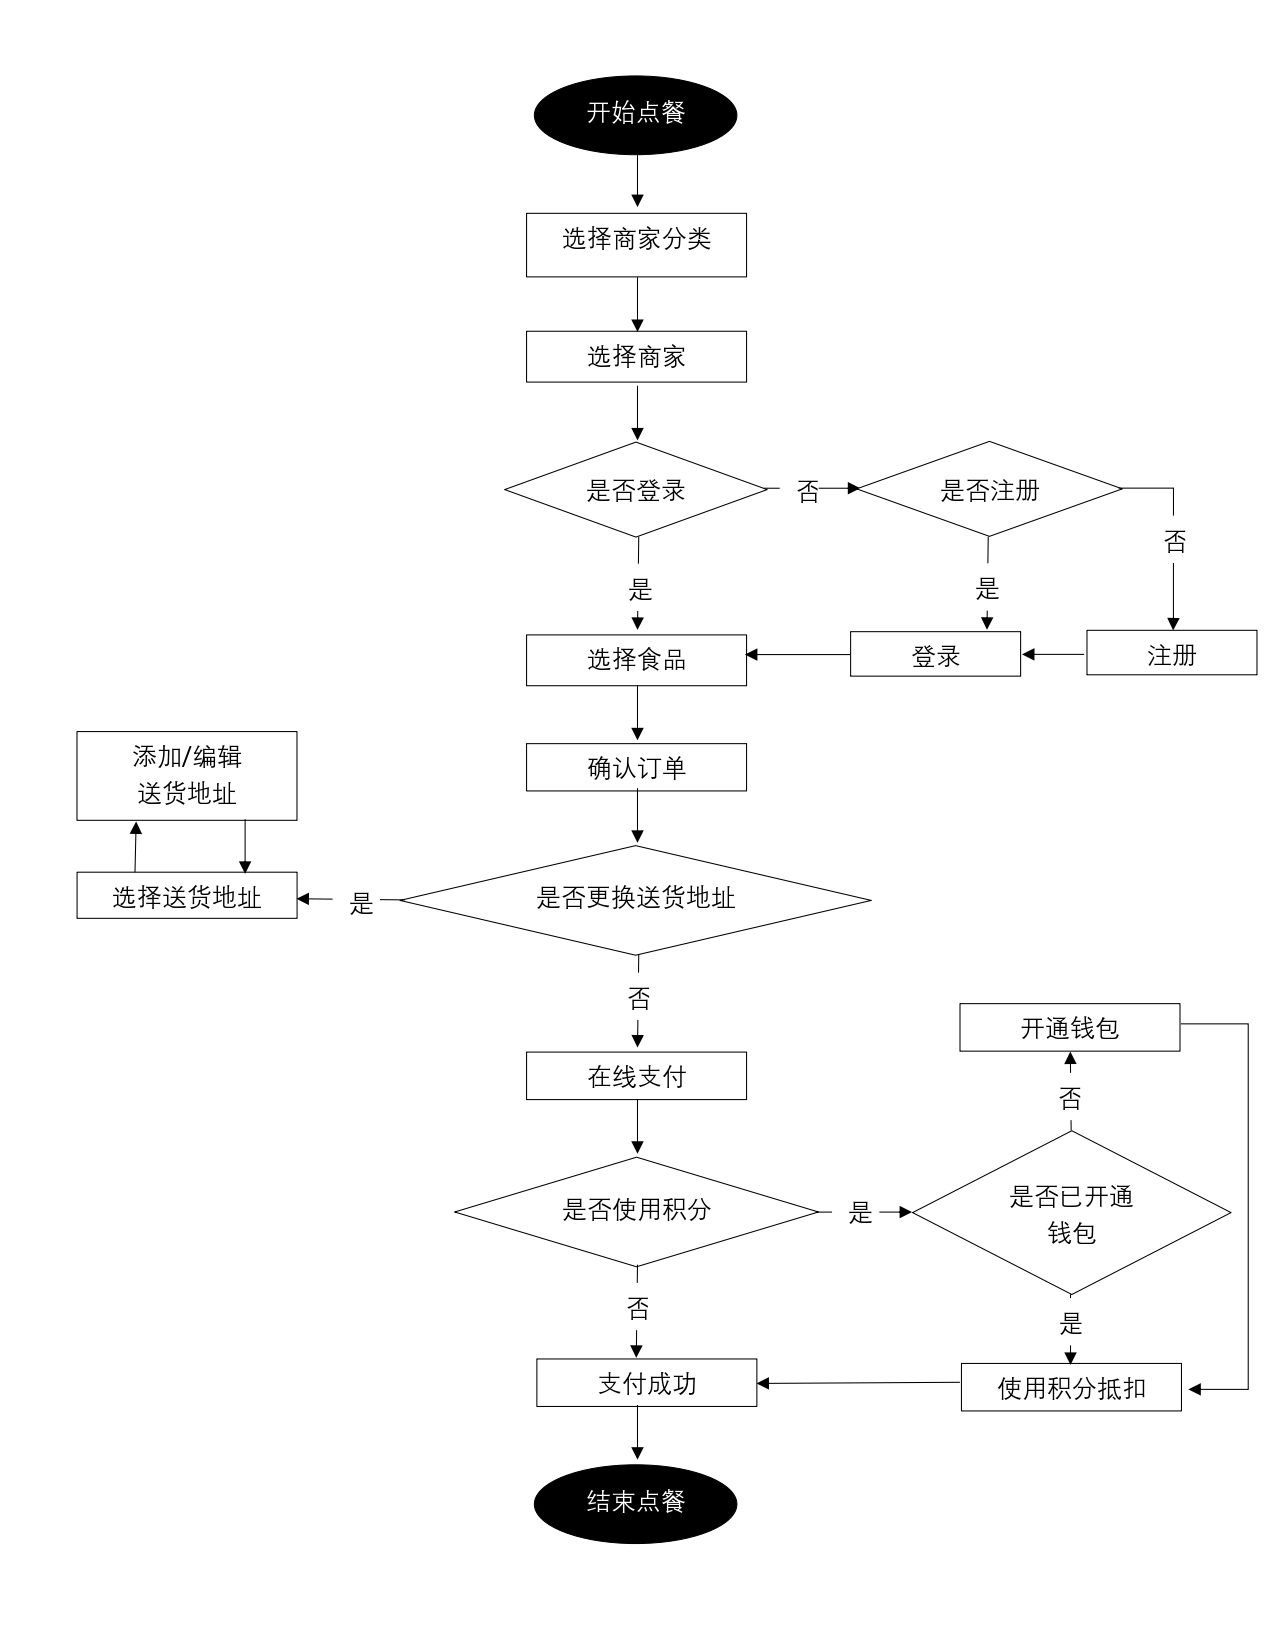
\includegraphics[width=0.8\textwidth]{processmap}
    \caption{饿了么外卖平台用户点餐业务流程图}\label{fig:process}
    \vspace{\baselineskip}
    \end{figure}

\section{用户需求}
本软件由三个用户组成,分别为用户、商家和管理员。用户角色由表~\ref{tab:table1}~所示。
\begin{table}[htbp]
\caption{饿了么外卖平台不同用户的功能描述}\label{tab:table1}
\vspace{0.5em}\wuhao
\begin{tabularx}{\textwidth}{llX}
\toprule[1.5pt]
序号 & 用户 & 功能描述 \\ 
\midrule[1pt]
1 & 用户 & 
\begin{itemize}
    \item{\textbf{游览菜品}}:消费者可以在首页浏览附近的餐厅列表。他们可以按照菜系、评分、特别优惠等条件筛选餐厅,了解每家餐厅的菜单和菜品详情。
    \item{\textbf{选择菜品}}:消费者可以根据菜品的图片、描述以及价格做出最合适的选择。
    \item{\textbf{在线支付}}:消费者将所选的菜品添加到购物车,确认订单后选择第三方的支付方式进行支付,完成订单。
    \item {\textbf{管理地址信息}}:消费者可以自行添加、删除和查看收获地址的信息。
    \item {\textbf{管理订单信息}}:消费者可以在历史订单页面查看已生成的订单状态,其中包含已选购的商家和菜品明细。
    \item {\textbf{登陆注册}}:消费者可以通过手机号注册一个饿了么外卖平台的账号。
\end{itemize}
\\
2 & 商家 & 
\begin{itemize}
    \item{\textbf{注册和上架}}:商家需要先在平台上注册自己的餐厅。一旦注册成功,他们可以填写餐厅的基本信息、菜单、菜品描述和价格等。
    \item{\textbf{菜单管理}}:商家可以通过平台管理菜单,包括添加新菜品、修改菜品信息、调整价格等。
    \item{\textbf{接受订单}}:商家在平台上收到订单通知后,可以查看订单详情,包括所点菜品、数量、送达地址以及支付信息。
    \item {\textbf{准备食物}}:商家接受订单后,就可以开始准备食物。
\end{itemize}
\\
3 & 管理员 & 
\begin{itemize}
    \item{\textbf{平台监督和管理}}:管理员负责监督外卖平台的整体运营情况。他们使用管理后台工具,监控平台的性能、稳定性和安全性,确保用户能够顺利访问平台。
    \item{\textbf{监控订单和投诉}}:管理员跟踪订单处理流程,确保订单按时送达。
    \item{\textbf{技术支持和升级}}:管理员负责监督技术团队,确保平台的技术架构和功能持续适应市场需求,并在必要时进行系统更新。
    \item {\textbf{风险管理和安全性}}:管理员制定隐私政策、安全措施,确保用户的个人信息和支付数据得到妥善保护。
\end{itemize}
\\
\bottomrule[1.5pt]
\end{tabularx}
\vspace{\baselineskip}
\end{table}

\section{功能性需求}
\subsection{首页}
首页是本软件的主要页面。此页面展示了用户当前的收货地址、商家搜索栏、菜品分类、推荐商家列表以及其他优惠部分。首页的底部有一个菜单,显示外卖平台的【首页】、【发现】、【订单】以及【我的】按钮。用户可以点击相应的按钮跳转至对应的页面进行操作。
\subsubsection{界面设计}
本软件的首页界面设计如图~\ref{fig:index}~所示。
\begin{figure}[htbp]
\centering
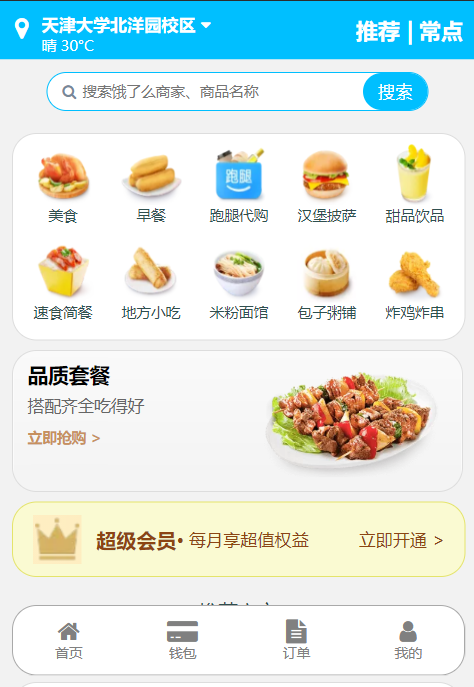
\includegraphics[width=0.4\textwidth]{index}
\caption{首页界面设计}\label{fig:index}
\vspace{\baselineskip}
\end{figure}
\subsubsection{功能按钮}
本软件首页功能按钮如表~\ref{tab:table2}~所示。
\begin{table}[htbp]
    \caption{饿了么外卖平台首页功能按钮}\label{tab:table2}
    \vspace{0.5em}\wuhao
    \begin{tabularx}{\textwidth}{lllX}
    \toprule[1.5pt]
    序号 & 按钮名称 & 功能 & 功能规则 \\ 
    \midrule[1pt]
    1 & 当前送货地址 & 用户选择送货地址 & 点击跳转至地址管理页面。 \\
    2 & 搜索框 & 用户搜索商家名称 & 输入商家名称可根据商家名称查找商家。 \\
    3 & 商家分类 & 用户选择商家分类 & 点击跳转指定商家分类。 \\
    4 & 首页 & 刷新页面 & 点击跳转至首页。 \\
    5 & 订单 & 进入历史订单 & 点击跳转至历史订单页面。 \\
    6 & 我的 & 进入用户信息 & 点击跳转至用户信息页面。 \\
\bottomrule[1.5pt]
\end{tabularx}
\vspace{\baselineskip}
\end{table}

\subsection{商家列表}
当用户在首页点击指定的商家分类后,会跳转至指定分类的商家列表页面。此页面展示了一系列商家,其中包括他们的商家图片、商家名称、商家的起送费、配送费和菜品。
\subsubsection{界面设计}
本软件的商家列表界面设计如图~\ref{fig:businessList}~所示。
\begin{figure}[htbp]
\centering
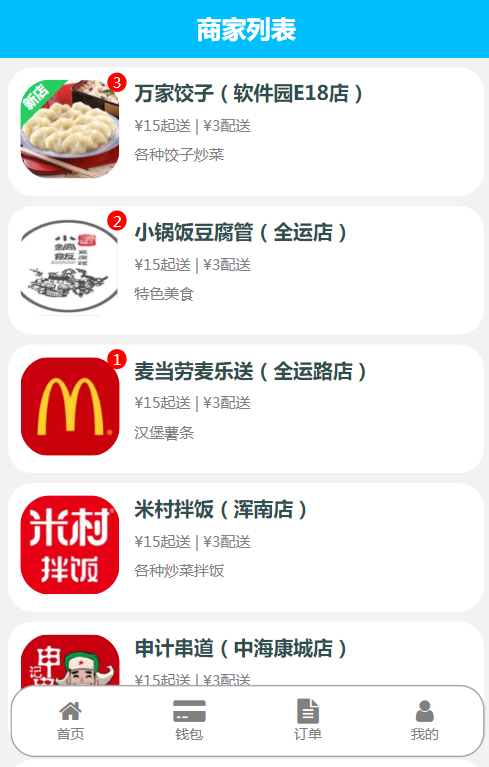
\includegraphics[width=0.4\textwidth]{businessList}
\caption{商家列表界面设计}\label{fig:businessList}
\vspace{\baselineskip}
\end{figure}
\subsubsection{功能按钮}
本软件商家列表功能按钮如表~\ref{tab:table3}~所示。
\begin{table}[htbp]
    \caption{饿了么外卖平台商家列表功能按钮}\label{tab:table3}
    \vspace{0.5em}\wuhao
    \begin{tabularx}{\textwidth}{lllX}
    \toprule[1.5pt]
    序号 & 按钮名称 & 功能 & 功能规则 \\ 
    \midrule[1pt]
    1 & 商家信息 & 用户选择指定商家 & 点击跳转至指定商家信息页面。 \\
    2 & 首页 & 刷新页面 & 点击跳转至首页。 \\
    3 & 订单 & 进入历史订单 & 点击跳转至历史订单页面。 \\
    4 & 我的 & 进入用户信息 & 点击跳转至用户信息页面。 \\
\bottomrule[1.5pt]
\end{tabularx}
\vspace{\baselineskip}
\end{table}

\subsection{商家信息}
当用户在商家列表页面中点击指定的商家后,会跳转至该商家的信息页面。此页面展示了该商家的图片、名称、起送费、配送费以及该商家一系列的菜品。此页面的下方显示了当前购物车的菜品数量、总价格以及【去结算】的按钮。
\subsubsection{界面设计}
本软件的商家信息界面设计如图~\ref{fig:businessInfo}~所示。
\begin{figure}[htbp]
\centering
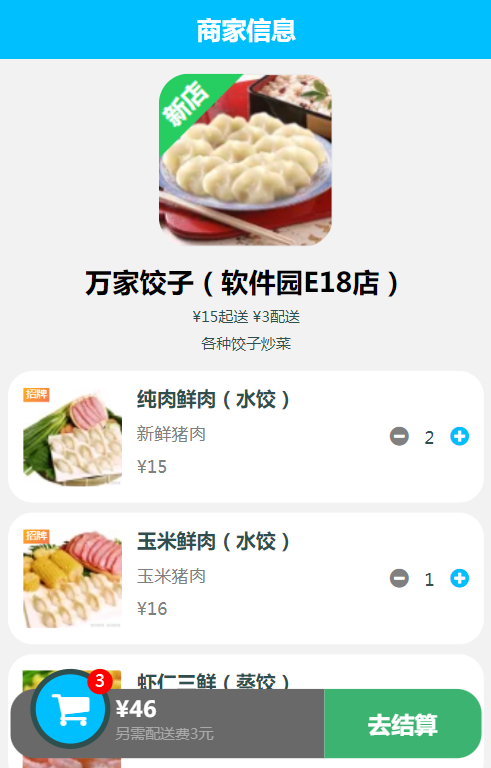
\includegraphics[width=0.4\textwidth]{businessInfo}
\caption{商家信息界面设计}\label{fig:businessInfo}
\vspace{\baselineskip}
\end{figure}
\subsubsection{功能按钮}
本软件商家信息功能按钮如表~\ref{tab:table4}~所示。
\begin{table}[htbp]
    \caption{饿了么外卖平台商家信息功能按钮}\label{tab:table4}
    \vspace{0.5em}\wuhao
    \begin{tabularx}{\textwidth}{lllX}
    \toprule[1.5pt]
    序号 & 按钮名称 & 功能 & 功能规则 \\ 
    \midrule[1pt]
    1 & 添加菜品 & 用户添加该菜品数量 & 点击将该菜品在购物车里的数量加1。 \\
    2 & 减少菜品 & 用户减少该菜品数量 & 点击将该菜品在购物车里的数量减1。 \\
    3 & 去结算 & 进入确认订单页面 & 点击会生成订单,跳转至确认订单页面。 \\
\bottomrule[1.5pt]
\end{tabularx}
\vspace{\baselineskip}
\end{table}

\subsection{确认订单}
当用户在商家信息页面中点击【去结算】按钮后,会跳转至确认订单页面。此页面展示了当前用户的送货地址、用户名称和手机号。在用户信息的下方显示了商家名称、购物车中所选择的菜品图片、菜品名称、菜品数量和配送费。在此页面的底部显示了总价格和【去支付】的按钮。
\subsubsection{界面设计}
本软件的确认订单界面设计如图~\ref{fig:order}~所示。
\begin{figure}[htbp]
\centering
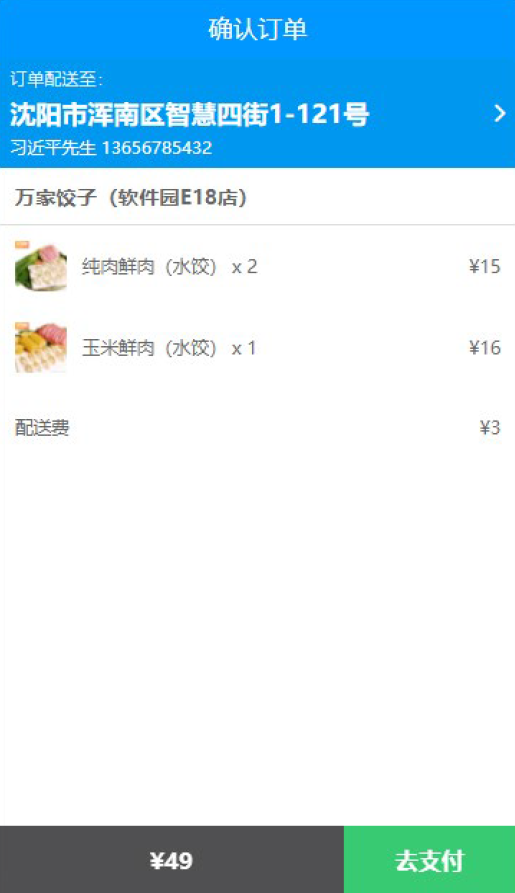
\includegraphics[width=0.4\textwidth]{order}
\caption{确认订单界面设计}\label{fig:order}
\vspace{\baselineskip}
\end{figure}
\subsubsection{功能按钮}
本软件确认订单功能按钮如表~\ref{tab:table5}~所示。
\begin{table}[htbp]
    \caption{饿了么外卖平台确认订单功能按钮}\label{tab:table5}
    \vspace{0.5em}\wuhao
    \begin{tabularx}{\textwidth}{lllX}
    \toprule[1.5pt]
    序号 & 按钮名称 & 功能 & 功能规则 \\ 
    \midrule[1pt]
    1 & 当前送货地址 & 用户选择送货地址 & 点击跳转至地址管理页面。 \\
    2 & 去支付 & 进入在线支付页面 & 点击跳转至在线支付页面。 \\
\bottomrule[1.5pt]
\end{tabularx}
\vspace{\baselineskip}
\end{table}

\subsection{在线支付}
当用户在确认订单页面中点击【去结算】按钮后,会跳转至确认订单页面。
\subsubsection{界面设计}
本软件的在线支付界面设计如图~\ref{fig:payment}~所示。
\begin{figure}[htbp]
\centering
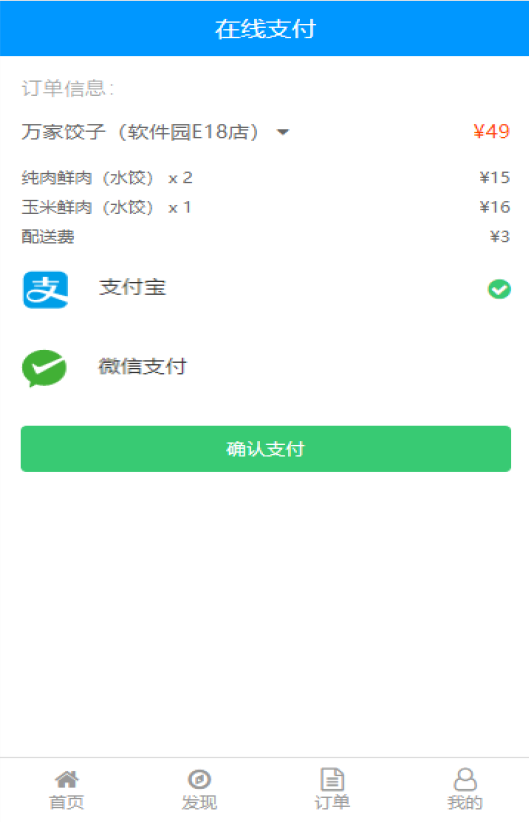
\includegraphics[width=0.4\textwidth]{payment}
\caption{在线支付界面设计}\label{fig:payment}
\vspace{\baselineskip}
\end{figure}
\subsubsection{功能按钮}
本软件在线支付功能按钮如表~\ref{tab:table6}~所示。
\begin{table}[htbp]
    \caption{饿了么外卖平台在线支付功能按钮}\label{tab:table6}
    \vspace{0.5em}\wuhao
    \begin{tabularx}{\textwidth}{lllX}
    \toprule[1.5pt]
    序号 & 按钮名称 & 功能 & 功能规则 \\ 
    \midrule[1pt]
    1 & 箭头 & 用户展开订单明细 & 点击展开已生成的订单明细,包括菜品的数量和价格。 \\
    2 & 选择支付方式 & 用户选择第三方的支付方式 & 点击选择任一第三方支付方式。 \\
    3 & 确认支付 & 用户支付订单 & 点击完成点餐流程。 \\
    4 & 首页 & 进入首页 & 点击跳转至首页。 \\
    5 & 订单 & 进入历史订单 & 点击跳转至历史订单页面。 \\
    6 & 我的 & 进入用户信息 & 点击跳转至用户信息页面。 \\
\bottomrule[1.5pt]
\end{tabularx}
\vspace{\baselineskip}
\end{table}

\subsection{用户登录}
此页面为用户登录的页面。用户需要输入手机号和密码,若两者正确无误则登陆成功并跳转至上一个页面,否则服务器将会提示信息错误。
\subsubsection{界面设计}
本软件的用户登录界面设计如图~\ref{fig:login}~所示。
\begin{figure}[htbp]
\centering
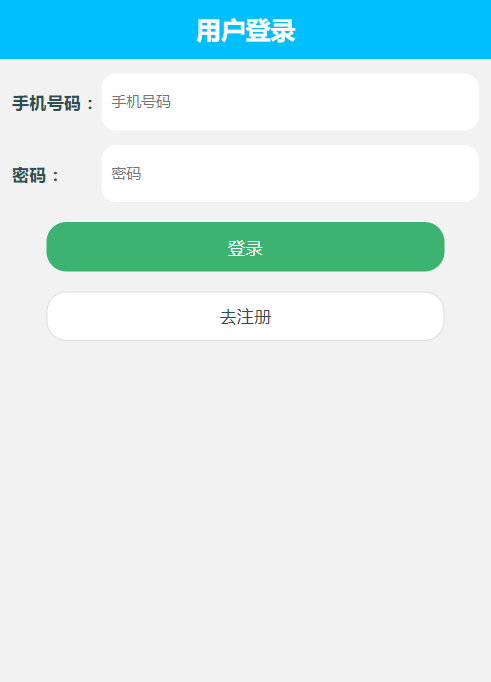
\includegraphics[width=0.4\textwidth]{login}
\caption{用户登录界面设计}\label{fig:login}
\vspace{\baselineskip}
\end{figure}
\subsubsection{功能按钮}
本软件用户登录功能按钮如表~\ref{tab:table7}~所示。
\begin{table}[htbp]
    \caption{饿了么外卖平台用户登录功能按钮}\label{tab:table7}
    \vspace{0.5em}\wuhao
    \begin{tabularx}{\textwidth}{lllX}
    \toprule[1.5pt]
    序号 & 按钮名称 & 功能 & 功能规则 \\ 
    \midrule[1pt]
    1 & 登录 & 用户登录 & 若手登陆成功则跳转至上一个页面,否则服务器将会显示错误提示。 \\
    2 & 去注册 & 用户注册 & 点击跳转至用户注册页面。 \\
    3 & 首页 & 进入首页 & 点击跳转至首页。 \\
    4 & 订单 & 进入历史订单 & 点击跳转至历史订单页面。 \\
    5 & 我的 & 进入用户信息 & 点击跳转至用户信息页面。 \\
\bottomrule[1.5pt]
\end{tabularx}
\vspace{\baselineskip}
\end{table}

\subsection{用户注册}
此页面为用户注册的页面。用户需要输入手机号、两次相同的密码、用户姓名以及选择性别。若手机号、密码和用户名都符合要求,则注册成功并跳转至登陆页面,否则服务器将会提示信息错误。
\subsubsection{界面设计}
本软件的用户注册界面设计如图~\ref{fig:register}~所示。
\begin{figure}[htbp]
\centering
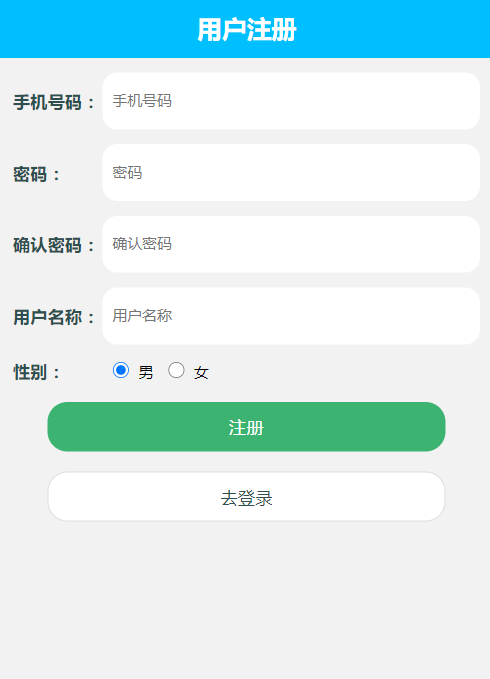
\includegraphics[width=0.4\textwidth]{register}
\caption{用户注册界面设计}\label{fig:register}
\vspace{\baselineskip}
\end{figure}
\subsubsection{功能按钮}
本软件用户注册功能按钮如表~\ref{tab:table8}~所示。
\begin{table}[htbp]
    \caption{饿了么外卖平台用户注册功能按钮}\label{tab:table8}
    \vspace{0.5em}\wuhao
    \begin{tabularx}{\textwidth}{lllX}
    \toprule[1.5pt]
    序号 & 按钮名称 & 功能 & 功能规则 \\ 
    \midrule[1pt]
    1 & 性别 & 用户选择性别 & 点击选择任一性别。 \\
    2 & 注册 & 用户注册 & 若注册成功则跳转至登陆页面,否则服务器将显示错误提示。 \\
    3 & 首页 & 进入首页 & 点击跳转至首页。 \\
    4 & 订单 & 进入历史订单 & 点击跳转至历史订单页面。 \\
    5 & 我的 & 进入用户信息 & 点击跳转至用户信息页面。 \\
\bottomrule[1.5pt]
\end{tabularx}
\vspace{\baselineskip}
\end{table}

\subsection{历史订单}
历史订单页面展示了用户之前所生成的全部订单,未支付的订单会显示在页面的上方,已支付的订单则会显示在页面的下方。
\subsubsection{界面设计}
本软件的历史订单界面设计如图~\ref{fig:orderList}~所示。
\begin{figure}[htbp]
\centering
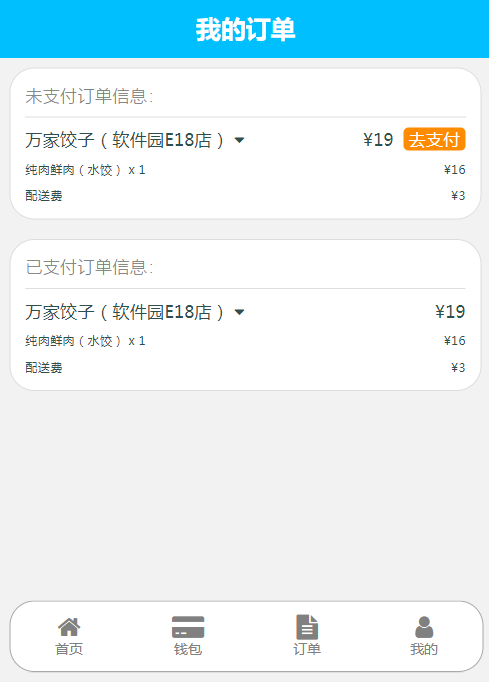
\includegraphics[width=0.4\textwidth]{orderList}
\caption{历史订单界面设计}\label{fig:orderList}
\vspace{\baselineskip}
\end{figure}
\subsubsection{功能按钮}
本软件历史订单功能按钮如表~\ref{tab:table9}~所示。
\begin{table}[htbp]
    \caption{饿了么外卖平台历史订单功能按钮}\label{tab:table9}
    \vspace{0.5em}\wuhao
    \begin{tabularx}{\textwidth}{lllX}
    \toprule[1.5pt]
    序号 & 按钮名称 & 功能 & 功能规则 \\ 
    \midrule[1pt]
    1 & 箭头 & 用户展开订单明细 & 点击展开已生成的订单明细,包括菜品的数量和价格。 \\
    2 & 去支付 & 用户支付未支付的订单 & 点击跳转至未支付的订单页面。 \\
    3 & 首页 & 进入首页 & 点击跳转至首页。 \\
    4 & 订单 & 刷新页面 & 点击跳转至历史订单页面。 \\
    5 & 我的 & 进入用户信息 & 点击跳转至用户信息页面。 \\
\bottomrule[1.5pt]
\end{tabularx}
\vspace{\baselineskip}
\end{table}

\subsection{地址管理}
当用户在首页或在确认订单页面点击送货地址按钮时,会跳转到此页面。此页面显示了用户的所有送货地址。
\subsubsection{界面设计}
本软件的地址管理界面设计如图~\ref{fig:userAddress}~所示。
\begin{figure}[htbp]
\centering
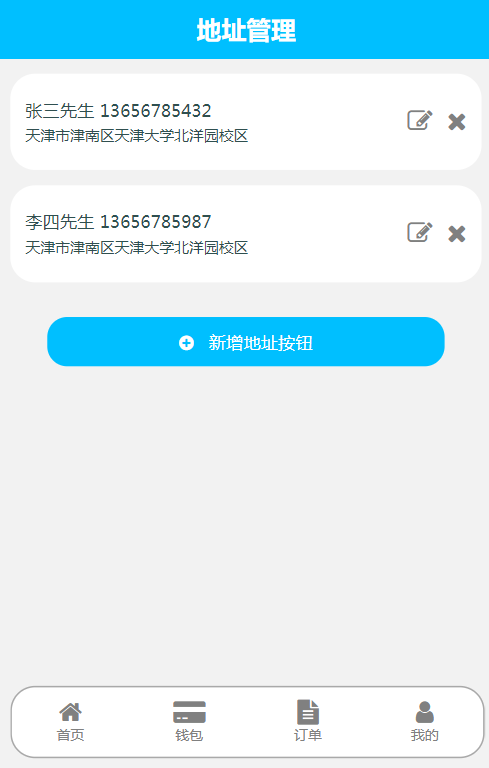
\includegraphics[width=0.4\textwidth]{userAddress}
\caption{地址管理界面设计}\label{fig:userAddress}
\vspace{\baselineskip}
\end{figure}
\subsubsection{功能按钮}
本软件地址管理功能按钮如表~\ref{tab:table10}~所示。
\begin{table}[htbp]
    \caption{饿了么外卖平台地址管理功能按钮}\label{tab:table10}
    \vspace{0.5em}\wuhao
    \begin{tabularx}{\textwidth}{lllX}
    \toprule[1.5pt]
    序号 & 按钮名称 & 功能 & 功能规则 \\ 
    \midrule[1pt]
    1 & 送货地址 & 用户选择该送货地址 & 点击选择该送货地址,并跳转至上一个页面。 \\
    2 & 编辑图标 & 用户编辑该送货地址 & 点击跳转至编辑送货地址页面。 \\
    3 & 打叉图标 & 用户删除该送货地址 & 点击删除该送货地址,地址管理页面减少该送货地址。 \\
    4 & 新增收货地址 & 用户添加送货地址 & 点击跳转至新增送货地址页面。 \\
    5 & 首页 & 进入首页 & 点击跳转至首页。 \\
    6 & 订单 & 进入历史订单 & 点击跳转至历史订单页面。 \\
    7 & 我的 & 进入用户信息 & 点击跳转至用户信息页面。 \\
\bottomrule[1.5pt]
\end{tabularx}
\vspace{\baselineskip}
\end{table}

\subsection{新增送货地址}
用户在此页面添加新的送货地址。填写完成后,点击保存按钮跳转至地址管理页面。
\subsubsection{界面设计}
本软件的新增送货地址界面设计如图~\ref{fig:addUserAddress}~所示。
\begin{figure}[htbp]
\centering
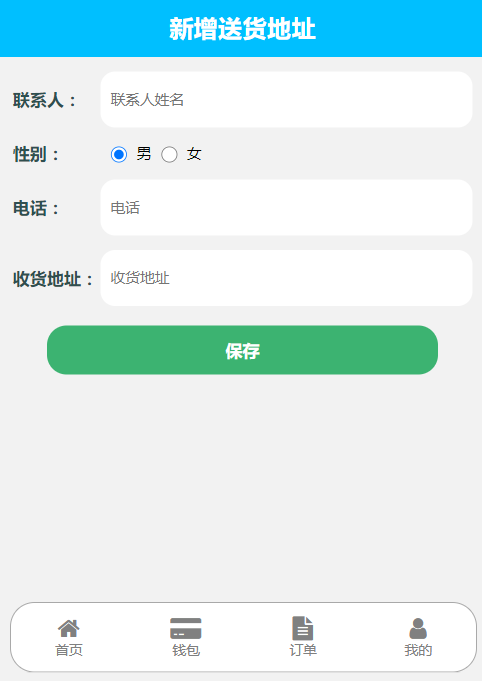
\includegraphics[width=0.4\textwidth]{addUserAddress}
\caption{新增送货地址界面设计}\label{fig:addUserAddress}
\vspace{\baselineskip}
\end{figure}
\subsubsection{功能按钮}
本软件新增送货地址功能按钮如表~\ref{tab:table11}~所示。
\begin{table}[htbp]
    \caption{饿了么外卖平台新增送货地址功能按钮}\label{tab:table11}
    \vspace{0.5em}\wuhao
    \begin{tabularx}{\textwidth}{lllX}
    \toprule[1.5pt]
    序号 & 按钮名称 & 功能 & 功能规则 \\ 
    \midrule[1pt]
    1 & 性别 & 用户选择性别 & 点击选择任一性别。 \\
    2 & 保存 & 用户保存当前送货地址 & 点击跳转至地址管理页面。 \\
    3 & 首页 & 进入首页 & 点击跳转至首页。 \\
    4 & 订单 & 进入历史订单 & 点击跳转至历史订单页面。 \\
    5 & 我的 & 进入用户信息 & 点击跳转至用户信息页面。 \\
\bottomrule[1.5pt]
\end{tabularx}
\vspace{\baselineskip}
\end{table}

\subsection{编辑地址}
用户在此页面编辑已选择的送货地址。填写完成后,点击保存按钮跳转至地址管理页面。
\subsubsection{界面设计}
本软件的编辑送货地址界面设计如图~\ref{fig:editUserAddress}~所示。
\begin{figure}[htbp]
\centering
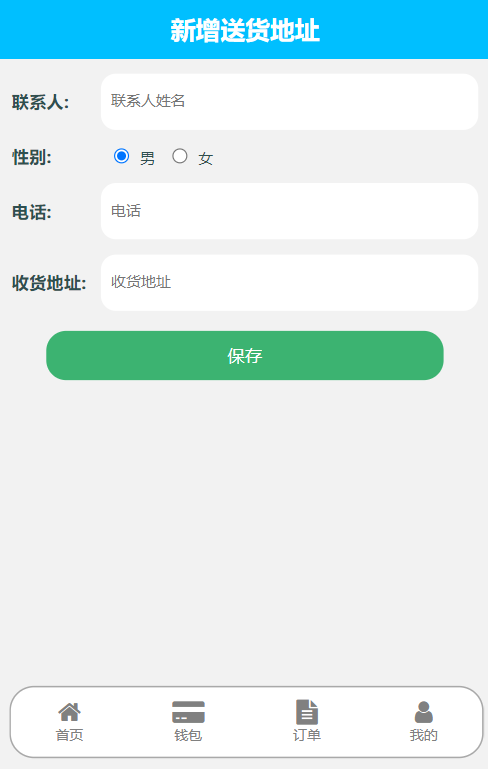
\includegraphics[width=0.4\textwidth]{editUserAddress}
\caption{编辑送货地址界面设计}\label{fig:editUserAddress}
\vspace{\baselineskip}
\end{figure}
\subsubsection{功能按钮}
本软件编辑送货地址功能按钮如表~\ref{tab:table12}~所示。
\begin{table}[htbp]
    \caption{饿了么外卖平台编辑送货地址功能按钮}\label{tab:table12}
    \vspace{0.5em}\wuhao
    \begin{tabularx}{\textwidth}{lllX}
    \toprule[1.5pt]
    序号 & 按钮名称 & 功能 & 功能规则 \\ 
    \midrule[1pt]
    1 & 性别 & 用户选择性别 & 点击选择任一性别。 \\
    2 & 保存 & 用户保存当前送货地址 & 点击跳转至地址管理页面。 \\
    3 & 首页 & 进入首页 & 点击跳转至首页。 \\
    4 & 订单 & 进入历史订单 & 点击跳转至历史订单页面。 \\
    5 & 我的 & 进入用户信息 & 点击跳转至用户信息页面。 \\
\bottomrule[1.5pt]
\end{tabularx}
\vspace{\baselineskip}
\end{table}

\subsection{个人信息}
个人信息页面显示当前用户的图片和名称。用户可以在此页面修改用户名和密码、跳转至地址管理页面以及退出登录。
\subsubsection{界面设计}
本软件的个人信息界面设计如图~\ref{fig:profile}~所示。
\begin{figure}[htbp]
\centering
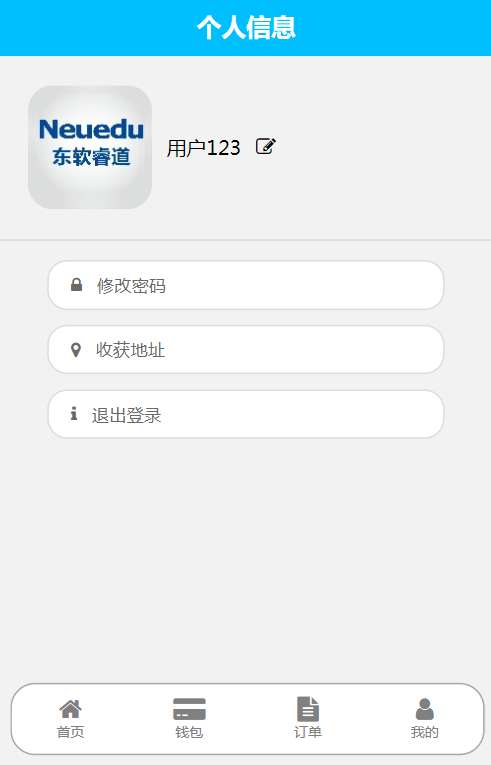
\includegraphics[width=0.4\textwidth]{profile}
\caption{个人信息界面设计}\label{fig:profile}
\vspace{\baselineskip}
\end{figure}
\subsubsection{功能按钮}
本软件编辑送货地址功能按钮如表~\ref{tab:table13}~所示。
\begin{table}[htbp]
    \caption{饿了么外卖平台编辑送货地址功能按钮}\label{tab:table13}
    \vspace{0.5em}\wuhao
    \begin{tabularx}{\textwidth}{lllX}
    \toprule[1.5pt]
    序号 & 按钮名称 & 功能 & 功能规则 \\ 
    \midrule[1pt]
    1 & 编辑图标 & 进入更新用户名页面 & 点击跳转至更新用户名页面。 \\
    2 & 修改密码 & 进入更新密码页面 & 点击跳转至更新密码页面。 \\
    3 & 收货地址 & 进入地址管理页面 & 点击跳转至地址管理页面。 \\
    4 & 退出登录 & 进入首页 & 点击退出登录,跳转至首页。 \\
    5 & 首页 & 进入首页 & 点击跳转至首页。 \\
    6 & 订单 & 进入历史订单页面 & 点击跳转至历史订单页面。 \\
    7 & 我的 & 刷新页面 & 点击跳转至用户信息页面。 \\
\bottomrule[1.5pt]
\end{tabularx}
\vspace{\baselineskip}
\end{table}

\subsection{更新用户名}
用户在此页面更新用户名。填写完成后,点击保存按钮跳转至个人信息页面。
\subsubsection{界面设计}
本软件的更新用户名界面设计如图~\ref{fig:updateUserName}~所示。
\begin{figure}[htbp]
\centering
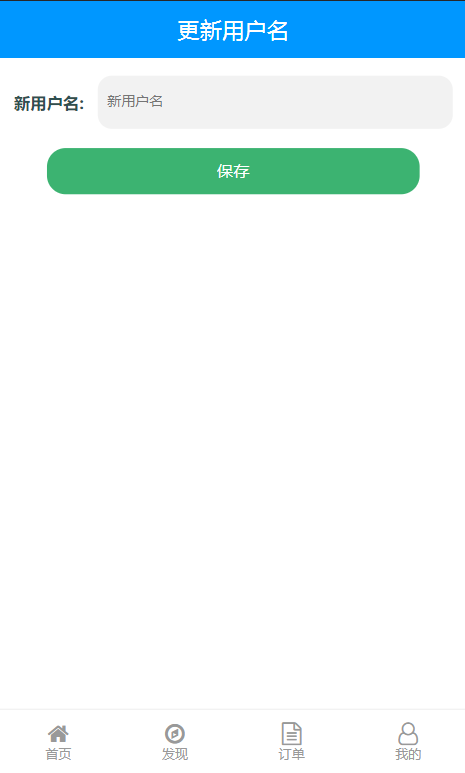
\includegraphics[width=0.4\textwidth]{updateUserName}
\caption{更新用户名界面设计}\label{fig:updateUserName}
\vspace{\baselineskip}
\end{figure}
\subsubsection{功能按钮}
本软件更新用户名功能按钮如表~\ref{tab:table14}~所示。
\begin{table}[htbp]
    \caption{饿了么外卖平台更新用户名功能按钮}\label{tab:table14}
    \vspace{0.5em}\wuhao
    \begin{tabularx}{\textwidth}{lllX}
    \toprule[1.5pt]
    序号 & 按钮名称 & 功能 & 功能规则 \\ 
    \midrule[1pt]
    1 & 保存 & 用户保存当前用户名 & 点击跳转至个人信息页面。 \\
    2 & 首页 & 进入首页 & 点击跳转至首页。 \\
    3 & 订单 & 进入历史订单页面 & 点击跳转至历史订单页面。 \\
    4 & 我的 & 刷新页面 & 点击跳转至用户信息页面。 \\
\bottomrule[1.5pt]
\end{tabularx}
\vspace{\baselineskip}
\end{table}

\subsection{更新密码}
用户在此页面更新密码。填写完成后,点击保存按钮跳转至个人信息页面。
\subsubsection{界面设计}
本软件的更新密码界面设计如图~\ref{fig:updateUserPassword}~所示。
\begin{figure}[htbp]
\centering
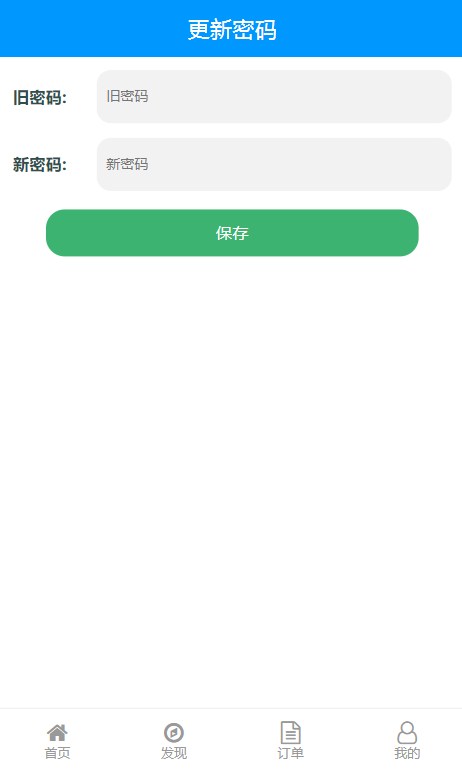
\includegraphics[width=0.4\textwidth]{updateUserPassword}
\caption{更新密码界面设计}\label{fig:updateUserPassword}
\vspace{\baselineskip}
\end{figure}
\subsubsection{功能按钮}
本软件更新密码功能按钮如表~\ref{tab:table15}~所示。
\begin{table}[htbp]
    \caption{饿了么外卖平台更新密码功能按钮}\label{tab:table15}
    \vspace{0.5em}\wuhao
    \begin{tabularx}{\textwidth}{lllX}
    \toprule[1.5pt]
    序号 & 按钮名称 & 功能 & 功能规则 \\ 
    \midrule[1pt]
    1 & 保存 & 用户保存当前密码 & 点击跳转至个人信息页面。 \\
    2 & 首页 & 进入首页 & 点击跳转至首页。 \\
    3 & 订单 & 进入历史订单页面 & 点击跳转至历史订单页面。 \\
    4 & 我的 & 刷新页面 & 点击跳转至用户信息页面。 \\
\bottomrule[1.5pt]
\end{tabularx}
\vspace{\baselineskip}
\end{table} %项目需求
	% \chapter{JDBC~项目}

\section{设计}

\section{测试}

\section{部署} %第一项目
	% \chapter{前端项目}

\section{设计}
\subsection{项目相关知识点}
\subsubsection{屏幕视口}
移动端的屏幕尺寸非常多样,而不像~PC~端的屏幕那样一致。因此,在移动设备上显示网页时,由于尺寸的不同,可能会出现网页内容显示不全且需要横向滚动的情况,因此在本软件运用了屏幕视口(viewport)的功能。

屏幕视口可分为三种,分别为:
\begin{enumerate}
    \item{布局视口(layout viewport)}:网页的实际尺寸。
    \item {理想视口(ideal viewport)}:网页在屏幕上的实际尺寸,根据机型的不同,尺寸也不尽相同。
    \item {视觉视口(visual viewport)}:用户所能看到的视口范围。
\end{enumerate}

通过使用屏幕视口(viewport),可以有效解决上述的问题:将网页放置在布局视口(layout viewport)中,然后按比例缩小布局视口以适应理想视口(ideal viewport)。这样可以确保无论网页的内容如何,都能在移动设备的屏幕上完整显示,而且不会出现横向滚动条的情况。

在每次开发网页前,我们会在头部加上一段屏幕视口的代码,代码如下:
\begin{lstlisting}[basicstyle=\footnotesize]
<meta name="viewport" content="width=device-width, initial-scale=1">
\end{lstlisting}
其中,~width~是布局视口,而~device-width~理想尺寸。因此,~width=device-width~就是将布局视口按照理想视口的实际尺寸来显示。

\subsubsection{弹性布局}
在此项目中,我们会将某些元素(div)的~display~属性值设置为~flex~,那么这个元素就可以称为是一个弹性布局容器(弹性容器)。它的子元素将会按照弹性布局的规则来排列和对齐。
\begin{lstlisting}[basicstyle=\footnotesize]
display: flex
\end{lstlisting}

在弹性布局中,默认存在着两根轴,分别是水平方向的主轴和垂直方向的侧轴。如图~\ref{fig:axis}~所示。
\begin{figure}[htbp]
    \centering
    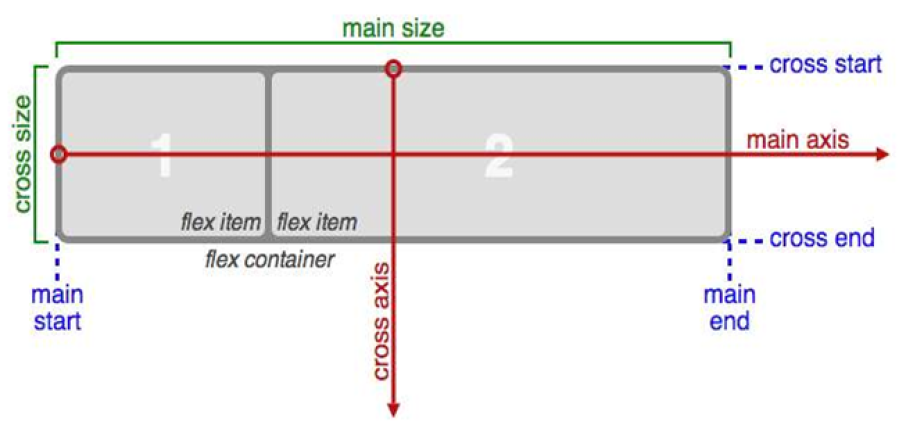
\includegraphics[width=0.8\textwidth]{axis}
    \caption{弹性布局的主轴与侧轴}\label{fig:axis}
    \vspace{\baselineskip}
\end{figure}

我们使用~flex-direction~属性来设置主轴的方向,row~为主轴方向且为默认值,而column~为侧轴方向。
\begin{lstlisting}[basicstyle=\footnotesize]
flex-direction: column
\end{lstlisting}

由于弹性布局中的子元素能自动伸缩,因此当父容器的尺寸小于子元素整体尺寸时,子元素会自动收缩,而不是自动换行。如果向让子元素自动换行,需要使用~flex-wrap: wrap。
\begin{lstlisting}[basicstyle=\footnotesize]
display: flex
flex-wrap: wrap
\end{lstlisting}

在此项目中,我们会设置 justify-content 样式,让子元素水平居中、居右等等。其中,justify-content 有五种值:
\begin{enumerate}
    \item{flex-start}:居左,为默认值。
    \item {flex-end}:居右。
    \item {center}:居中。
    \item {space-between}:两端对齐,每个子元素的间距相等。
    \item {space-around}:每个子元素两侧的间距相等。
\end{enumerate}
\begin{lstlisting}[basicstyle=\footnotesize]
display: flex
justify-content: space-between
\end{lstlisting}

除了让子元素水平居中、居右等,我们还使用了 align-items 样式,以让子元素垂直居中。
\begin{lstlisting}[basicstyle=\footnotesize]
display: flex
align-items: center
\end{lstlisting}

为了让每个子元素所占空间不一致,我们也使用 flex 样式给子元素按比例分配空间。如果设置了 flex,width 与 height 就会失效。
\begin{lstlisting}[basicstyle=\footnotesize]
<body>
    <div class="son" style="flex:1;">1</div>
    <div class="son" style="flex:1;">2</div>
    <div class="son" style="flex:2;">3</div>
</body>
\end{lstlisting}
在上面例子中,三个 div 的宽度分别是窗口宽度的 1/4、1/4 和 1/2。
\begin{lstlisting}[basicstyle=\footnotesize]
<body>
    <div class="son" style="flex:0 0 400px;">1</div>
    <div class="son" style="flex:1;">2</div>
    <div class="son" style="flex:2;">3</div>
</body>
\end{lstlisting}
在上面例子中,第一个 div 的宽度是 400px,是不变的。第二个和第三个 div 将剩下宽度按比例分配:1/3、2/3。

在移动端中,视口指的是屏幕视口中的布局视口。视口尺寸常用的有 vw 和 vh。1vw 等于视口宽度的1\%,而 1vh 等于视口高度的1\%。在此项目中,我们会多使用 vw,以实现元素宽度按移动端当前的宽度自动缩放。
\begin{lstlisting}[basicstyle=\footnotesize]
<style>
    div{
        width: 30vw;
        height: 20vw;
        background-color: blue;
        color: #fff;
        font-size: 5vw;
    }
</style>
\end{lstlisting}

CSS3 新增了 border-box 的盒子模型,即宽和高为边框。我们使用 box-sizing 的属性来设置盒子模型类型。使用了边框盒子后,就可以任意设置内边距、边框,不需要担心会改变盒子的总体尺寸。
\begin{lstlisting}[basicstyle=\footnotesize]
div{
    width: 200px;
    height: 200px;
    box-sizing: border-box; 
    padding: 30px;
    border: solid 30px blue;
    margin: 50px;
}
\end{lstlisting}

\subsection{项目搭建}
本项目为前端静态页面项目,一共制作 15 个不同的页面,分别为:
\begin{enumerate}
    \item{首页}
    \item {商家列表页面}
    \item {商家信息页面}
    \item {确认订单页面}
    \item {在线支付页面}
    \item {支付成功页面}
    \item {历史订单页面}
    \item {地址管理页面}
    \item {新增地址页面}
    \item {编辑地址页面}
    \item {用户登录页面}
    \item {用户注册页面}
    \item {个人信息页面}
    \item {更新用户名页面}
    \item {更新密码页面}
\end{enumerate}

本项目可分为三个部分,分别为相应页面的 HTML 部分、CSS 部分和 JavaScript 三个部分。在项目文件中,也存放了 framework 文件和 img 文件,前者为存放第三方库字体图标库以及 CSS 重置文件;后者则为存放网页所需要插入的一些图片。本项目的文件如图~\ref{fig:part2folder}~所示。

我们使用了 font-awesome 作为本软件的第三方字体图标库,让我们可以插入各种不同的图标,以增加用户对于本软件的视觉效果。Font-awesome 第三方字体图标库网页如图~\ref{fig:fontawesomeweb}~所示。

创建 CSS 重置文件主要是为了去除 CSS 默认的边角、列表样式以及超链接下划线,代码如下:
\begin{lstlisting}[basicstyle=\footnotesize]
/* ----------------CSS 重置-------------- */
html, body, div, span, h1, h2, h3, h4, h5, h6, ul, ol, li, p{
    margin: 0;
    padding: 0;
}
/* 将边角去掉 */
html, body{
    height: 100%;
    weight: 100%;
    font-family: "微软雅黑";
}
/* 去掉列表样式 */
ul,ol{
    list-style: none;
}
/* 去掉超链接下划线 */
a{
     text-decoration: none;
}
\end{lstlisting}
\begin{figure}[htbp]
    \centering
    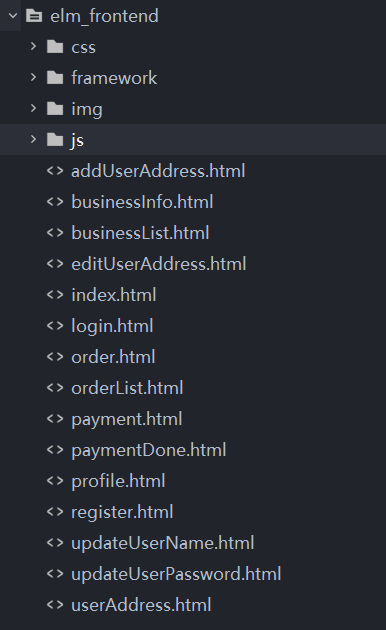
\includegraphics[width=0.4\textwidth]{part2folder}
    \caption{项目结构}\label{fig:part2folder}
    \vspace{\baselineskip}
\end{figure}
\begin{figure}[htbp]
    \centering
    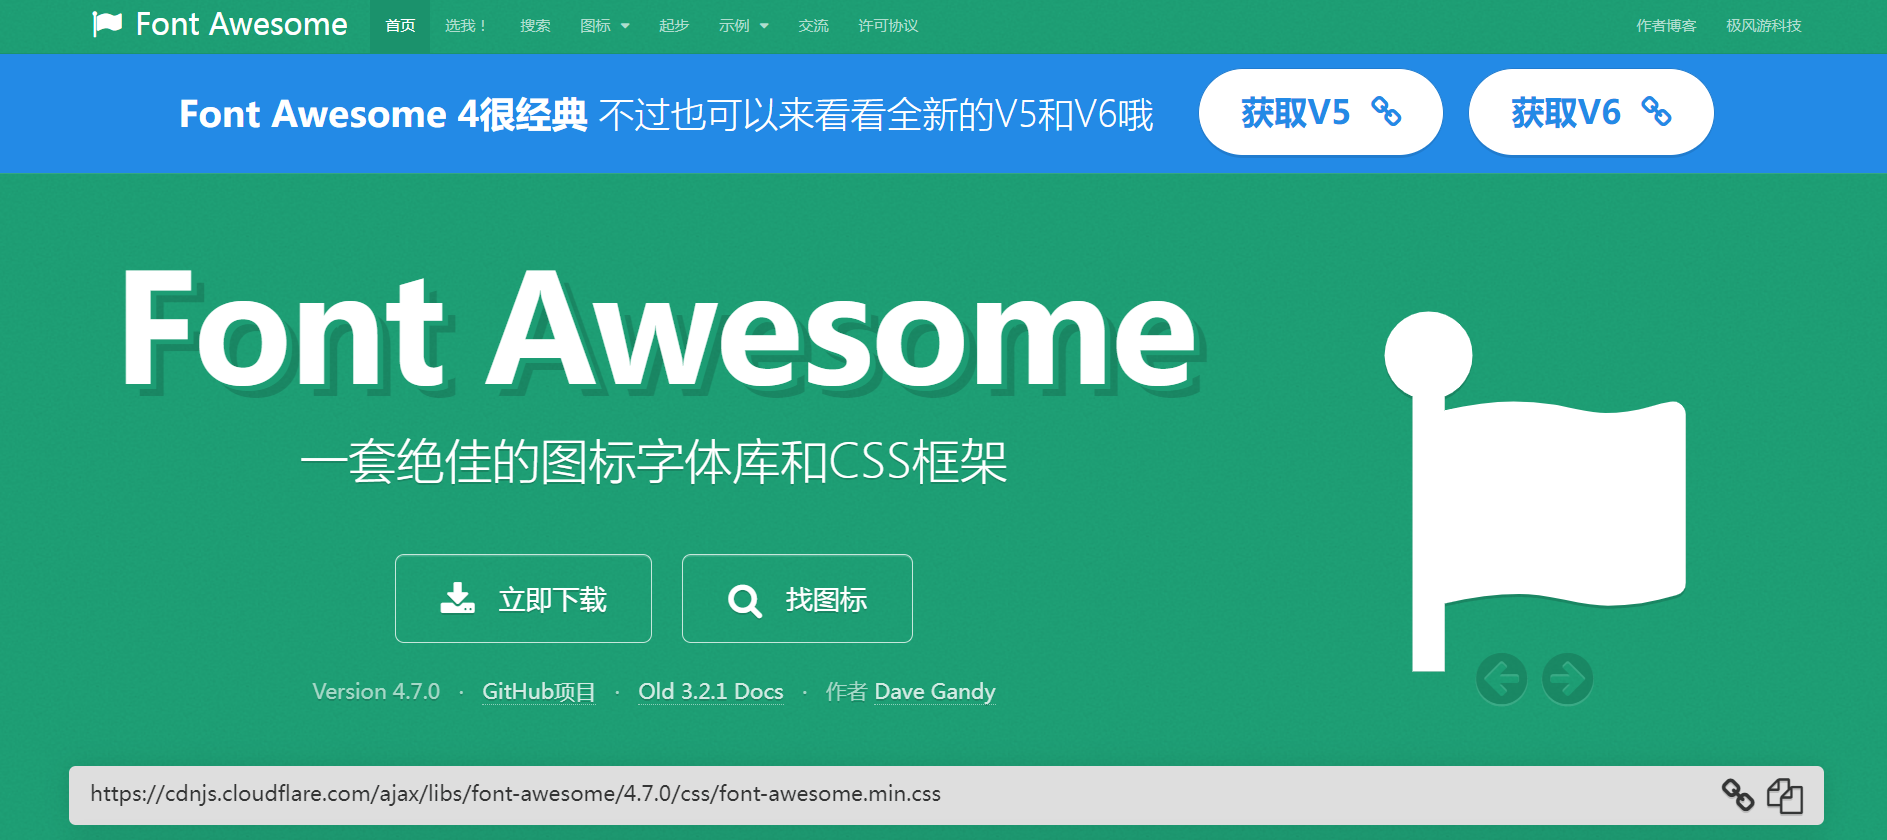
\includegraphics[width=0.8\textwidth]{fontawesomeweb}
    \caption{Font-awesome 网页}\label{fig:fontawesomeweb}
    \vspace{\baselineskip}
\end{figure}

\subsection{共通部分}
本软件的页面采用了共通的头部设计,因此在每个页面的 HTML 和 CSS 文件中都会包含这些共通部分的代码。
\subsubsection{页面头部}
对于每个页面,都采用了相同的页面头部,其中头部尺寸、背景色以及字体都是相同的。因此,在每个页面的 HTML 文件和 CSS 文件都会包含以下代码:
\begin{lstlisting}[basicstyle=\footnotesize]
/***** HTML 部分 *****/
<header><p>商家列表</p></header>

/***** CSS 部分 *****/
.wrapper header{
	width: 100%;
	height: 12vw;
	background-color: deepskyblue;
	position: fixed;
	top: 0;
	left: 0;
	display: flex;
	justify-content: center;
	align-items: center;
	color: white;
	font-size: 5vw;
	font-weight: 700;
}
\end{lstlisting}    
以上代码的生成结果如图~\ref{fig:headerfix}~所示。
\begin{figure}[htbp]
    \centering
    
\includegraphics[width=0.8\textwidth]{headerfix}
    \caption{页面头部界面设计}\label{fig:headerfix}
    \vspace{\baselineskip}
\end{figure}

\subsubsection{底部菜单}
除了商家列表页面、商家信息页面以及支付成功页面,对于每个页面也采用了相同的底部菜单设计。该底部菜单固定在屏幕的底部,但不会独占整个底部,而是稍微向上腾出一点空间,给予底部菜单一种悬浮的视觉效果。

因此,在这些页面的 HTML 和 CSS 文件中都会包含以下代码:
\begin{lstlisting}[basicstyle=\footnotesize]
/***** HTML 部分 *****/
<ul class="footer">
    <li onclick="location.href = 'index.html'">
        <i class="fa fa-home"></i>
        <p>首页</p>
    </li>
    <li>
        <i class="fa fa-compass"></i>
        <p>发现</p>
    </li>
    <li onclick="location.href = 'orderList.html'">
        <i class="fa fa-file-text"></i>
        <p>订单</p>
    </li>
    <li onclick="location.href = 'profile.html'">
        <i class="fa fa-user"></i>
        <p>我的</p>
    </li>
</ul>

/***** CSS 部分 *****/
.wrapper .footer{
	width: 95%;
	height: 14vw;
	border: solid 1.5px darkgray;
	background-color: white;
	border-radius: 5vw;
	position: fixed;
	bottom: 3vw;
	left: 2.5%;
	display:flex;
	justify-content: space-around;
	align-items: center;
}
.wrapper .footer li{
	display:flex;
	flex-direction: column;
	align-items: center;
	justify-content: center;
	font-size:5vw;
	color: gray;
	user-select: none;
	cursor: pointer;
}
.wrapper .footer li p{
	font-size:2.8vw;
}
\end{lstlisting}
以上代码的生成结果如图~\ref{fig:footerfix}~所示。  
\begin{figure}[htbp]
    \centering
    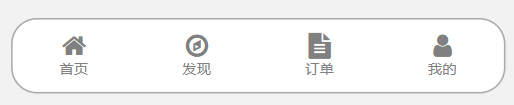
\includegraphics[width=0.8\textwidth]{footerfix}
    \caption{页面底部菜单界面设计}\label{fig:footerfix}
    \vspace{\baselineskip}
\end{figure}

\subsection{固定块}
本软件的页面主要有两个部分为固定块,分别为页面的底部菜单和首页中的搜索框部分。

\subsubsection{底部菜单}
对于页面的底部菜单,我们在相应页面的 CSS 文件中的底部菜单部分添加了 position: fixed 来达到固定屏幕上的效果。此外,为了呈现居中以及悬浮的效果,也增加了一段 left: 2.5\% 和 bottom: 3vw,其作用是为了让底部菜单向左保持 2.5\% 的间距以及向上移动 3vw。代码如下:
\begin{lstlisting}[basicstyle=\footnotesize]
position: fixed;
bottom: 3vw;
left: 2.5%;
\end{lstlisting}

\subsubsection{首页搜索框}
对于首页的搜索框部分,如果页面向下滑动,需要呈现出搜索框始终固定在头部的效果。这需要使用到 JavaScript 为搜索框写出一段逻辑代码。

我们使用了 onscroll 事件为固定搜索框创建一个函数。首先,我们获取滚动条的位置,获取PC端滚动条位置为 document.documentElement.scrollTop,而获取移动端滚动条位置为 document.body.scrollTop。由于 PC 端和移动端的获取方法有所不同,因此我们对它们做出了一个判断,如果从 PC 端获取的返回结果不为 0 则使用 PC 端的滚动条位置,否则使用移动端的滚动条位置。

接着,使用 document.documentElement.clientWidth 来获取视口的宽度,这对 PC 端和移动端都有效,然后使用 document.getElementById('fixedBox') 获取搜索框块。最后,写出一个判断:如果滚动条的位置大于首页头部的高度(12 vw),则将搜索框转换成固定,即写为 position: fixed;否则搜索框保持不变。代码如下:
\begin{lstlisting}[basicstyle=\footnotesize]
document.onscroll = function(){
    //获取滚动条位置
    let s1 = document.documentElement.scrollTop;
    let s2 = document.body.scrollTop;
    let scroll = s1==0?s2:s1; //判断是否是移动端或PC端
    //获取视口宽度
    let width = document.documentElement.clientWidth;
    //获取固定块
    let search = document.getElementById('fixedBox');
    if(scroll > width * 0.12){ //因为header的高度是 12vw
        search.style.position = 'fixed';
        search.style.left = '0';
        search.style.top = '0';
    }
    else{
        search.style.position = 'static';
    }
}
\end{lstlisting}
以上代码的执行效果如图~\ref{fig:searchnonfix}~和图~\ref{fig:searchfix}~所示。
\begin{figure}[htbp]
    \centering
    \begin{minipage}{0.4\textwidth}
    \centering
    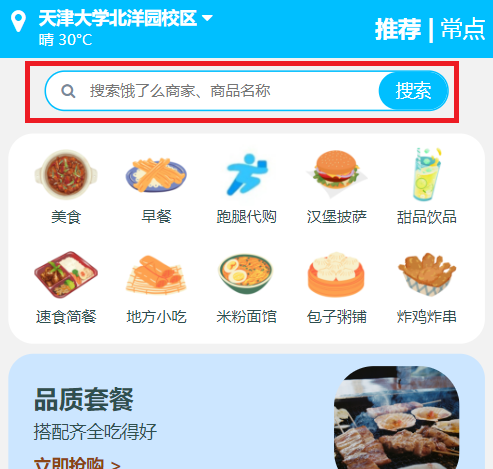
\includegraphics[width=\textwidth]{searchnonfix}
    \caption{首页无滚动时的搜索框}\label{fig:searchnonfix}
    \end{minipage}
    \begin{minipage}{0.4\textwidth}
    \centering
    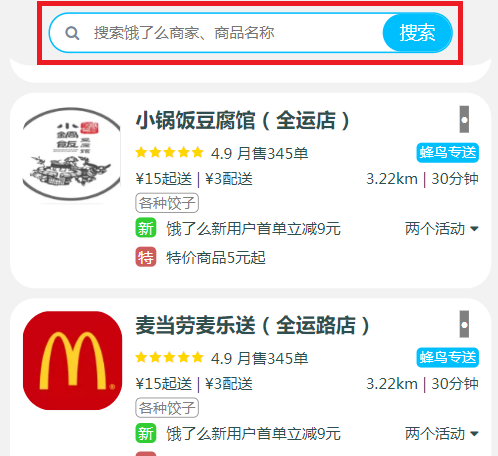
\includegraphics[width=\textwidth]{searchfix}
    \caption{首页滚动后的搜索框}\label{fig:searchfix}
    \end{minipage}
    \vspace{\baselineskip}
\end{figure}

\subsection{订单明细的显示与隐藏}
本软件有两个页面需要显示和隐藏外卖订单的明细,分别为确认订单页面以及历史订单页面。

首先,使用 document.getElementsByClassName('fa-caret-down') 和 document.getElementsByClassName('order-detail') 获取按钮和订单明细的对象。接着,使用 detailBox.style.display='none' 来初始化订单明细为隐藏状态。

最后,使用 onclick 事件为显示和隐藏订单明细的按钮创建一个函数。在函数里写出一个判断:如果当前订单明细为隐藏状态,则当点击按钮时会显示订单明细;否则点击按钮时会隐藏订单明细。代码如下:
\begin{lstlisting}[basicstyle=\footnotesize]
//获取显示隐藏按钮对象
let downBtn  = document.getElementsByClassName('fa-caret-down');
//获取隐藏订单明细对象
let detailBox = document.getElementsByClassName('order-detail');
//所有订单明细初始为隐藏状态
for(let i = 0; i < downBtn.length; i++){
    detailBox[i].style.display='none';
}
for(let i = 0; i < downBtn.length; i++){
    downBtn[i].onclick = function(){
        //判断隐藏订单明细是否隐藏
        if(detailBox[i].style.display=='none'){
            detailBox[i].style.display='block';
        }
        else{
            detailBox[i].style.display='none';
        }
    }
}
\end{lstlisting}
以上代码的执行效果如图~\ref{fig:orderhidden}~和图~\ref{fig:ordershown}~所示。
\begin{figure}[htbp]
    \centering
    \begin{minipage}{0.4\textwidth}
    \centering
    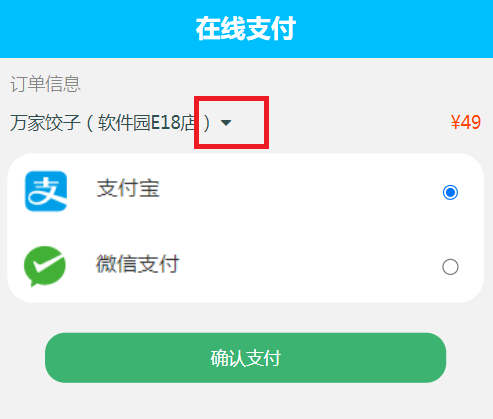
\includegraphics[width=\textwidth]{orderhidden}
    \caption{订单明细隐藏状态}\label{fig:orderhidden}
    \end{minipage}
    \begin{minipage}{0.4\textwidth}
    \centering
    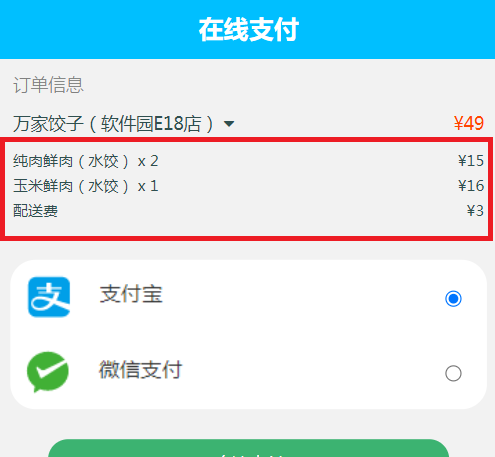
\includegraphics[width=\textwidth]{ordershown}
    \caption{订单明细显示状态}\label{fig:ordershown}
    \end{minipage}
    \vspace{\baselineskip}
\end{figure}

\section{测试}
对于本项目的测试,主要着重于每个页面的按钮是否能跳转至正确的页面,以及对于某些页面的逻辑操作是否正确。

\subsection{页面按钮测试}
对于页面按钮的测试,首先测试每个页面的底部菜单按钮是否都可以跳转至相应的页面。如果点击 “首页” 则必须跳转至首页;点击 “发现” 则没有任何效果;点击 “订单” 则必须跳转至历史订单页面;点击 “我的” 则必须跳转至个人信息页面。

经过测试,每个设计底部菜单的页面都可以正常跳转至指定的页面,如图~\ref{fig:part2test}~所示。
\begin{figure}[htbp]
    \centering
    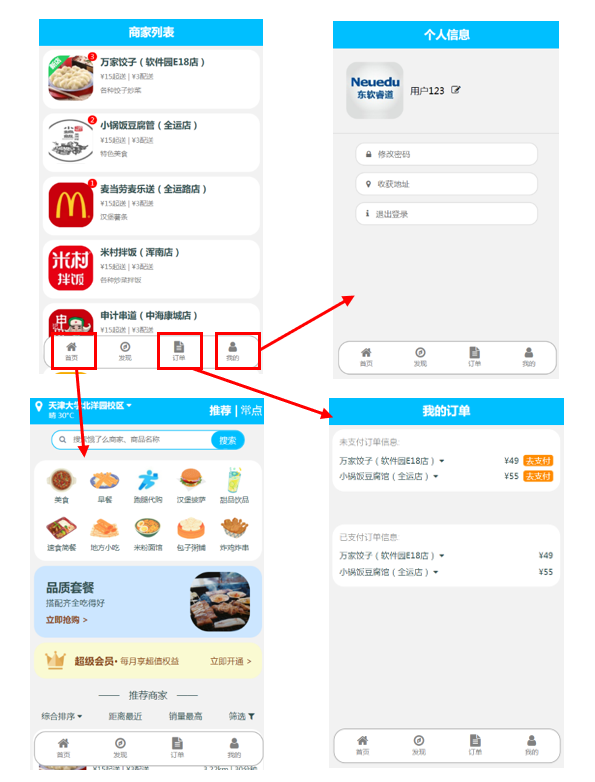
\includegraphics[width=0.5\textwidth]{part2test}
    \caption{页面底部菜单按钮测试}\label{fig:part2test}
    \vspace{\baselineskip}
\end{figure}

接着我们测试了其余页面的其他按钮是否可以正确跳转至相应的页面。由于本软件的按钮过多,因此在本项目的测试部分只显示首页、地址管理页面和个人信息页面的按钮测试结果,如图~\ref{fig:part2test1}~和图~\ref{fig:part2test2}~所示。
\begin{figure}[htbp]
    \begin{minipage}{0.6\textwidth}
    \centering
    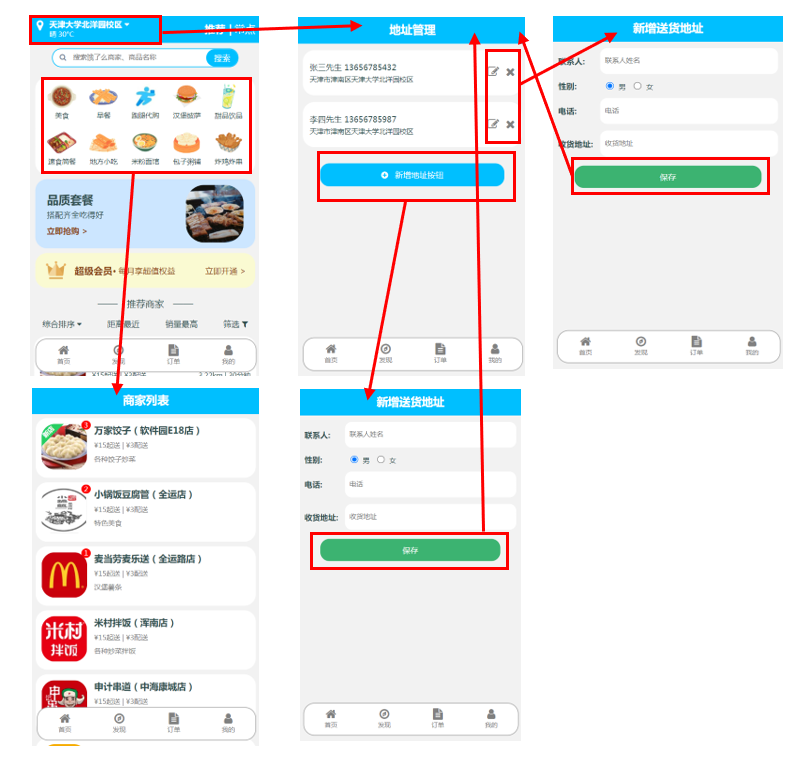
\includegraphics[width=\textwidth]{part2test1}
    \caption{首页和地址管理页面按钮测试}\label{fig:part2test1}
    \end{minipage}
    \begin{minipage}{0.5\textwidth}
    \centering
    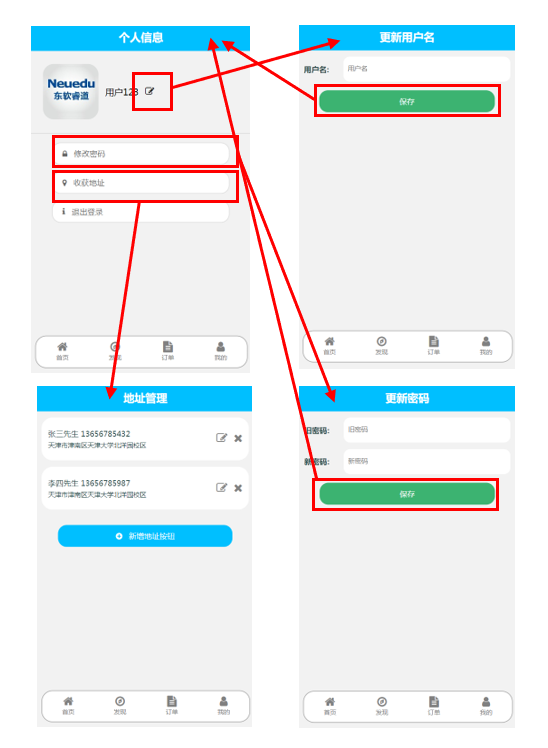
\includegraphics[width=\textwidth]{part2test2}
    \caption{个人信息页面按钮测试}\label{fig:part2test2}
    \end{minipage}
    \vspace{\baselineskip}
\end{figure}

\subsection{页面逻辑操作}
在本项目中需要对逻辑操作进行测试的页面有首页、确认订单页面与历史订单页面。对于首页,我们所需要测试的是搜索框在页面向下滑动时是否会固定在页面头部,测试结果如图~\ref{fig:part2test3}~和图~\ref{fig:part2test4}~所示。
\begin{figure}[htbp]
    \centering
    \begin{minipage}{0.4\textwidth}
    \centering
    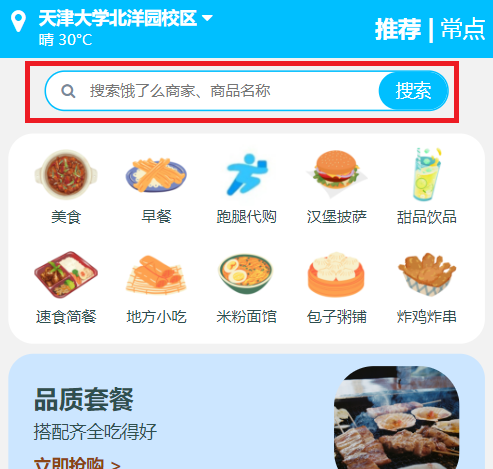
\includegraphics[width=\textwidth]{searchnonfix}
    \caption{首页无滚动时的搜索框}\label{fig:part2test3}
    \end{minipage}
    \begin{minipage}{0.4\textwidth}
    \centering
    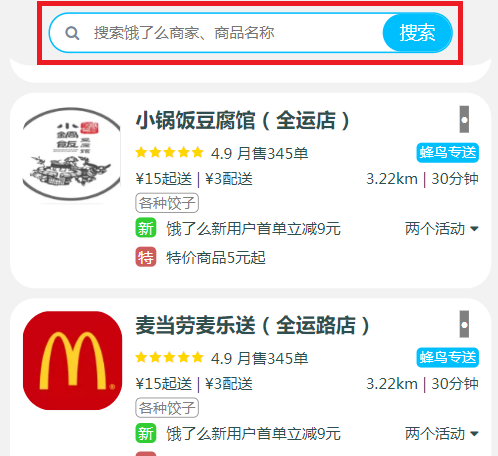
\includegraphics[width=\textwidth]{searchfix}
    \caption{首页滚动后的搜索框}\label{fig:part2test4}
    \end{minipage}
    \vspace{\baselineskip}
\end{figure}

接着,对于确认订单页面和历史订单页面,我们测试了这两个页面是否可以正确显示和隐藏订单,且在初始状态时为隐藏状态。测试结果如图~\ref{fig:part2test5}~至~\ref{fig:part2test8}~所示。
\begin{figure}[htbp]
    \centering
    \begin{minipage}{0.4\textwidth}
    \centering
    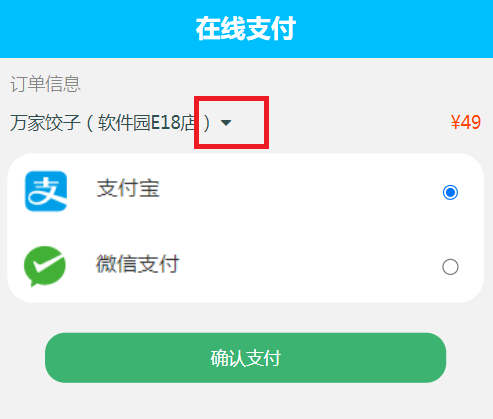
\includegraphics[width=\textwidth]{orderhidden}
    \caption{确认订单页面订单明细隐藏状态}\label{fig:part2test5}
    \end{minipage}
    \begin{minipage}{0.4\textwidth}
    \centering
    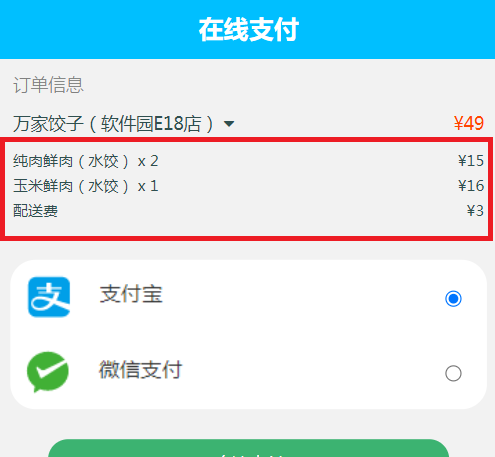
\includegraphics[width=\textwidth]{ordershown}
    \caption{确认订单页面订单明细显示状态}\label{fig:part2test6}
    \end{minipage}
    \vspace{\baselineskip}
\end{figure}
\begin{figure}[htbp]
    \centering
    \begin{minipage}{0.4\textwidth}
    \centering
    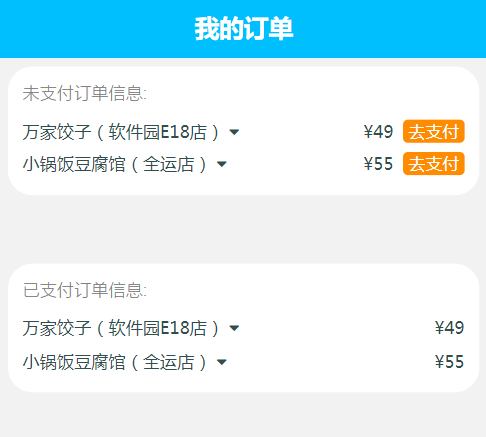
\includegraphics[width=\textwidth]{part2test7}
    \caption{历史订单页面订单明细隐藏状态}\label{fig:part2test7}
    \end{minipage}
    \begin{minipage}{0.4\textwidth}
    \centering
    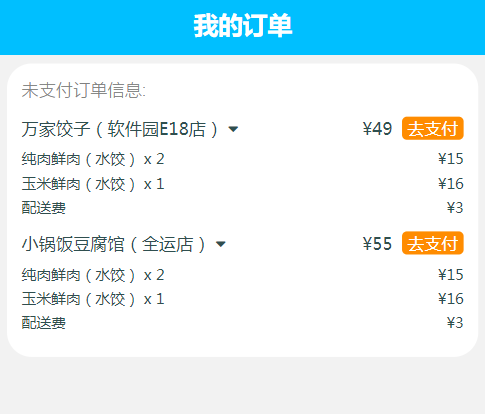
\includegraphics[width=\textwidth]{part2test8}
    \caption{历史订单页面订单明细显示状态}\label{fig:part2test8}
    \end{minipage}
    \vspace{\baselineskip}
\end{figure} %第二项目
	% \chapter{servlet项目}

\section{整体概述}
饿了么 Servlet 版项目是采用 VUE-CLI 与 Servlet 开发的前后端分离模式项目。前端Vue用于构建用户界面,同时在浏览器中发送XMLHttpRequest请求,
后端部分则致力于提供一套完整正确的用户点餐后端程序。

\section{项目技术架构}
VUE-CLI, JDK17, MySQL, Servlet, Tomcat8.5

\section{设计}
\subsection{功能描述}
支持用户完成整套点餐流程,包括选择商家,注册登录账户,修改账户信息,完成订单支付等功能。

\subsection{业务流程图}

\begin{figure}[htbp]
    \centering
    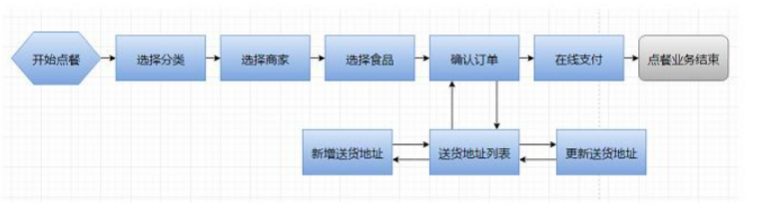
\includegraphics[width=0.8\textwidth]{servlet}
    \caption{servlet}
    \vspace{\baselineskip}
\end{figure}

\subsection{数据设计}
\subsubsection{实体类}

Business(商家)

私有变量:

商家ID:businessId(Integer)  商家名称:businessName(String)  密码:password(String)

商家地址:businessAddress(String)  商家描述信息:businessExplain(String)  起送费:starPrice(Double)

配送费:deliveryPrice(Double)  商家图片:businessImg(String)  商家类别:orderTypeId(Integer)  备注:remakrs(String))



Food(商品)

私有变量:

商品ID:foodId(Integer)  商品名:foodName(String)  商品描述信息:foodExplain(String)  价格:price(Double)

所属商家ID:businessId(Integer)  备注:remakrs(String)  商品图片:foodImg(String))



User(用户)

私有变量:

用户ID:userId(String)  用户名:userName(String)  密码:password(String)  性别:userSex(Integer)

用户头像:userImg(String)  删除标志:delTag(Integer))



Cart(购物车订单)

私有变量:

购物车订单Id:cartId(Integer)  商家ID:businessId(Integer)  商品ID:foodId(Integer)

用户ID:userId(String)  订购份数:quantity(Double))



DeliveryAddress(配送地址)

私有变量:

地址ID:daId(Integer)  联系人姓名:contactName(String)  联系人性别:contactSex(Integer)


联系人电话:contactTel  地址:address(String)  用户ID:userId(String))



Orders(订单)

私有变量:

订单Id:orderId(Integer)  用户ID:userId(String)  商家ID:businessId(Integer)


订单日期:orderDate(String)  订单金额:orderTotal(Double)  配送地址ID:daId(Integer)  订单状态:orderState(Integer))



OrderDetailet(订单明细)

私有变量:

订单明细ID:odId(Integer)  订单Id:orderId(Integer)  商品ID:foodId(Integer)  订单总量:quantity(Integer))

\subsubsection{工具类}
DBUtil(数据库连接工具):私有静态变量:DataSource(连接池工具,用来实现数据库持久连接)

CommonUtil(获取时间工具)

\subsection{数据库设计}

\begin{table}[htbp]
	\caption{商家表(点餐业务)}
	\vspace{0.5em}\wuhao
	\begin{tabularx}{\hsize}{@{\extracolsep{\fill}}c c c}
		\toprule[1.5pt]
		字段名          &  数据类型  &   说明 \\ 
		\midrule[1pt]
		businessId   & int  & 商家编号 \\
		businessName    & varchar  & 商家名称   \\
		businessAddress  & varchar & 商家地址 \\
		businessExplain     & varchar     & 商家介绍 \\
		businessImg      & mediumtext     & 商家图片 \\
		orderTypeId      & int     & 共用10种点餐分类 \\
		starPrice      & decimal     & 起送费 \\
		deliveryPrice      & decimal     & 配送费 \\
		remarks     & varchar     & 备注 \\
		\bottomrule[1.5pt]
	\end{tabularx}
	\vspace{\baselineskip}
\end{table}

\begin{table}[htbp]
	\caption{食品表(点餐业务)}
	\vspace{0.5em}\wuhao
	\begin{tabularx}{\hsize}{@{\extracolsep{\fill}}c c c}
		\toprule[1.5pt]
		字段名          &  数据类型  &   说明 \\ 
		\midrule[1pt]
		foodId      & int     & 食品编号 \\
		foodName   & varchar  & 食品名称 \\
		foodExplain    & varchar  & 食品介绍   \\
		foodImg      & mediumtext     & 食品图片 \\
		foodPrice      & decimal     & 食品价格 \\
		businessId      & int     & 所属商家编号 \\
		businessId      & varchar     & 备注 \\
		\bottomrule[1.5pt]
	\end{tabularx}
	\vspace{\baselineskip}
\end{table}

\begin{table}[htbp]
	\caption{购物车表}
	\vspace{0.5em}\wuhao
	\begin{tabularx}{\hsize}{@{\extracolsep{\fill}}c c c}
		\toprule[1.5pt]
		字段名          &  数据类型  &   说明 \\ 
		\midrule[1pt]
		cardId      & int     & 无意义编号 \\
		foodId   & int  & 食品名称 \\
		businessId    & int  & 所属商家编号   \\
		userId      & varchar     & 所属用户编号 \\
		quantity      & int     & 同一类型食品的购买数量 \\
		\bottomrule[1.5pt]
	\end{tabularx}
	\vspace{\baselineskip}
\end{table}

\begin{table}[htbp]
	\caption{送货地址表}
	\vspace{0.5em}\wuhao
	\begin{tabularx}{\hsize}{@{\extracolsep{\fill}}c c c}
		\toprule[1.5pt]
		字段名          &  数据类型  &   说明 \\ 
		\midrule[1pt]
		daId      & int     & 送货地址编号 \\
		contactName   & varchar  & 联系人姓名 \\
		contactSex    & int  & 联系人性别   \\
		contactTel   & varchar     & 联系人电话 \\
		address      & varchar     & 送货地址 \\
		userId      & varchar     & 所属用户编号 \\
		\bottomrule[1.5pt]
	\end{tabularx}
	\vspace{\baselineskip}
\end{table}

\begin{table}[htbp]
	\caption{订单表}
	\vspace{0.5em}\wuhao
	\begin{tabularx}{\hsize}{@{\extracolsep{\fill}}c c c}
		\toprule[1.5pt]
		字段名          &  数据类型  &   说明 \\ 
		\midrule[1pt]
		orderId      & int     & 订单编号 \\
		userId   & varchar  & 所属用户编号 \\
		businessId    & int  & 所属商家编号   \\
		orderDate   & varchar     & 订购日期 \\
		orderTotal      & decimal     & 订单总价 \\
		daId      & int     & 所属送货地址编号 \\
		orderState      & int     & 订单状态(0未支付,1已支付) \\
		\bottomrule[1.5pt]
	\end{tabularx}
	\vspace{\baselineskip}
\end{table}


\begin{table}[htbp]
	\caption{订单明细表}
	\vspace{0.5em}\wuhao
	\begin{tabularx}{\hsize}{@{\extracolsep{\fill}}c c c}
		\toprule[1.5pt]
		字段名          &  数据类型  &   说明 \\ 
		\midrule[1pt]
		odId      & int     & 订单明细编号 \\
		orderId   & int  & 所属订单编号 \\
		foodId    & int  & 所属食品编号   \\
		quantity   & int     & 数量 \\
		\bottomrule[1.5pt]
	\end{tabularx}
	\vspace{\baselineskip}
\end{table}

\begin{table}[htbp]
	\caption{用户表}
	\vspace{0.5em}\wuhao
	\begin{tabularx}{\hsize}{@{\extracolsep{\fill}}c c c}
		\toprule[1.5pt]
		字段名          &  数据类型  &   说明 \\ 
		\midrule[1pt]
		userId      & varchar     & 用户ID \\
		password   & varchar  & 密码 \\
		userName    & varchar  & 用户名   \\
		userSex      & int     & 性别 \\
		userImg      & mediumtext     & 用户头像 \\
		delTag      & int     & 删除标记 \\
		\bottomrule[1.5pt]
	\end{tabularx}
	\vspace{\baselineskip}
\end{table}

\subsection{程序结构}
项目三采用的MVC架构方式。

View:该模块是是负责与用户进行交互,向服务器发送用户请求,向用户发送服务器的回复。该层主要由前端部分完成。

Controller:该模块是将前前端发送的HTTP请求进行解析拆分,操作后端程序完成正确的相对应的操作。同时打包后端返回的消息成HTTP回复发送给前端。

Model:该模块是进行数据存储和数据库操作的部分。接受Controller发送的指令,对数据库进行相对应的操作,同时向Controler返回对应的消息。

\subsection{后端模块结构划分}
\subsubsection{Controller}
DispatcherServlet:处理前端发送过来的请求,将消息解析拆分发送给对应控制器的对应方法。也接收对应Controller发回的response,将它发回给前端。

Controller:接收前端控制器(DispatcherServlet)发来的请求,将其交付给Model模块处理请求,并接受Model发回的信息发回给DispatcherServlet。

\subsubsection{Model}
Service:被Controller层调用,并调用相对应的Dao层对数据库的操作方法,将相关信息发回给Controller。

Dao:对数据库进行相关操作,返回对应信息的层。

DB:后台数据库。

\subsection{结构图}

程序的结构图如图5-2所示:

\begin{figure}[htbp]
    \centering
    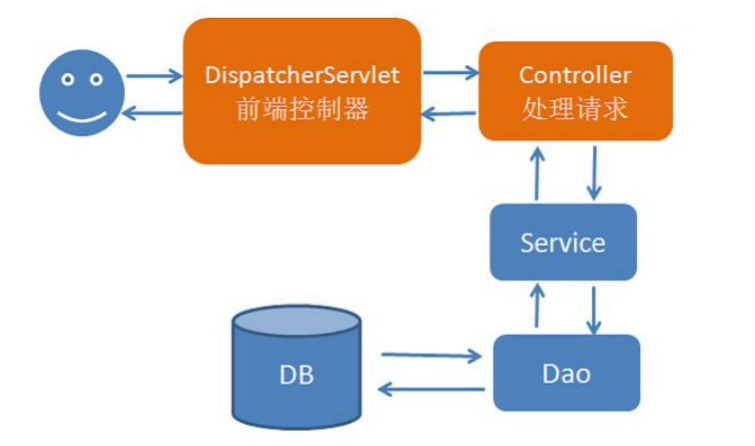
\includegraphics[width=0.8\textwidth]{MVC}
    \caption{MVC}\label{fig:MVC}
    \vspace{\baselineskip}
\end{figure}

\subsection{操作数据库接口描述}

\subsubsection{Admin}
\textbf{获取管理员对象}

getAdminByNameByPass

参数:adminName(String),password(String)

返回值:Admin

功能:传入管理员用户名和密码查找并返回对应的管理员实体。

\subsubsection{Business}
\textbf{列出相关商品类别的商家}

listBusinessByOrderTypeID

参数:orderTypeID(Integer)

返回值:List<Business>

功能:通过传入的商品类别列出此类别商家

\textbf{根据名搜索商家}

listBusinessByName

参数:businessName(String)

返回值:List<Business>

功能:通过输入字符串将商家名中含此字符串的商家列出

\textbf{根据地址搜索商家}

listBusinessByAddress

参数:businessAddress(String)

返回值:List<Business>

功能:通过输入字符串将商家字符串中含此字符串的商家列出

\textbf{获取商家}

getBusinessById

参数:businessId(Integer)

返回值:Business

功能:通过商家ID返回商家

\subsubsection{Food}
\textbf{列出商家商品}

listFoodByBusinessId

参数:businessId(Integer)

返回值:List<Food>

功能:查询数据库,列出商家ID对应商家的商品列表

\subsubsection{User}
\textbf{根据ID和密码返回账户}

getUserByIdByPass

参数:userId(String),password(String)

返回值:User

功能:根据输入的ID和密码返回对应账户

\textbf{查询账户}

getUserById

参数:userId(String)

返回值:int

功能:根据ID查询用户是否存在

\textbf{注册用户}

saveUser

参数:user(User)

返回值:int

功能:将传入的用户存入数据库

\textbf{更新用户名}

updateUserMsg

参数:userId(String),userName(String)

返回值:int

功能:修改对应ID的用户的用户名

\textbf{更新用户密码}

updateUserPassword

参数:userId(String),oldPass(String),newPass(String)

返回值:int

功能:判断密码是否正确。如果正确修改对应ID的用户的密码

\subsubsection{Cart}
\textbf{新建购物车账单}

saveCart

参数:cart(Cart)

返回值:int

功能:将传入的购物车账单存入数据库

\textbf{更新购物车}

updateCart

参数:cart(Cart)

返回值:int

功能:将与传入的购物车ID相同的购物车账单信息更新

\textbf{删除购物车账单}

removeCart

参数:cart(Cart)

返回值:int

功能:将与传入的购物车ID相同的购物车账单在数据库中删除

\textbf{列出购物车清单}

removeCart

参数:cart(Cart)

返回值:int

功能:如果存在businessId,列出对应user在此商家的购物车订单;如果不存在,列出此user所有的购物车账单

\subsubsection{DeliveryAddress}

\textbf{列出用户配送地址}

listDeliveryAddressByUserId

参数:userId(String)

返回值:List<DeliveryAddress>

功能:列出ID对应user的所有配送地址

\textbf{列出用户配送地址}

saveDeliveryAddress

参数:deliveryAddress(DeliveryAddress)

返回值:int

功能:将传入的地址存入数据库

\textbf{列出用户配送地址}

updateDeliveryAddress

参数:deliveryAddress(DeliveryAddress)

返回值:int

功能:将数据库中与传入参数daId相同的配送地址信息更新


\textbf{列出用户配送地址}

updateDeliveryAddress

参数:removeDeliveryAddress(DeliveryAddress)

返回值:int

功能:将数据库中与传入参数daId相同的配送地址删除

\textbf{根据地址ID查询地址}

getDeliveryAddressById

参数:daId(Integer)

返回值:DeliveryAddress

功能:将数据库中查询传对应daId的地址

\subsubsection{Orders}

\textbf{新建订单}

saveOrders

参数:orders(Orders)

返回值:int

功能:向数据库中存入传入的订单

\textbf{查询订单}

getOrdersById

参数:orderId(Integer)

返回值:Orders

功能:查询出与传入orderId相等的订单

\textbf{查询订单}

listOrdersByUserId

参数:userId(String)

返回值:List<Orders>

功能:列出与userId对应的用户的所有订单

\subsubsection{OrderDetailet}

\textbf{存储订单明细}

saveOrderDetailetBatch

参数:list(List<OrderDetailet>)

返回值:int

功能:将传入的订单明细组存入数据库

\textbf{存储订单明细}

listOrderDetailetByOrderId

参数:orderId(Integer)

返回值:List<OrderDetailet>

功能:列出所有数据库中与传入orderId相同的订单明细

\subsection{对外接口}
\textbf{处理http get方法}

DispatcherServlet/doGet

参数:request(HttpServletRequest) ,response(HttpServletResponse)

返回值:void

功能:处理发送的HTTP请求,将其发送给对应的Controller,让后端进行对应数据库操作,并将返回消息封装进response

\textbf{处理http Post方法}

DispatcherServlet/doPost

参数:request(HttpServletRequest) ,response(HttpServletResponse)

返回值:void

功能:处理发送的HTTP请求,将其发送给对应的Controller,让后端进行对应数据库操作,并将返回消息封装进response
\subsection{前端模块结构划分}
\begin{figure}[htbp]
    \centering
    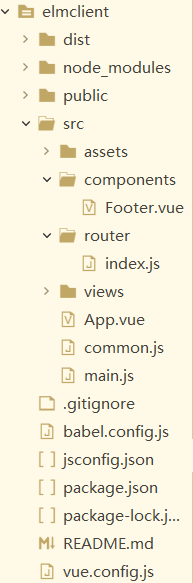
\includegraphics[width=0.4\textwidth,height=0.4\textheight]{vue1}
    \caption{前端模块结构}\label{fig:vue1}
\end{figure}
前端模块中,除了基本的项目依赖、配置文件外,主要是网页组件的制作。我们不仅需要根据不同的网页进行样式更改,还需要向服务端发送请求以获取数据资源,通过路由跳转来实现点餐过程中不同网页之间的切换。前端模块结构如图~\ref{fig:vue1}~所示

重要文件说明:
\begin{enumerate}
    \item {node\_modules文件夹}:用来存放用包管理工具下载安装的包,比如webpack、gulp、grunt这些工具。
    \item {assets文件夹}:存放网页制作所需的图片文件。
    \item {components/Footer.vue}:底部菜单组件。考虑到几乎所有页面都有底部菜单功能,为避免重复设计,我们将其单独存在Footer.vue中。在设计其他页面时,我们只需简单调用即可。
    \item {router/index.js}:路由配置文件。用来定义应用程序的路由规则,它包括了路由的基本配置信息,如路由路径、组件、重定向等,同时解决重复路由报异常的问题。
    \item {views文件夹}:用于存放不同的组件,每个组件对应一个网页。在组件中,template和style参考第四章前端项目的网页风格样式,script部分用于定义各种变量、方法,发送请求,对sessionStorage进行操作等。
    \item {App.vue}:存放共通样式,适用于所有组件。
    \item {common.js}:定义通用的方法,包括获取当前时间、向sessionStorage中增删改一个JSON对象、向localStorage中增删改一个JSON对象。
    \item {main.js}:项目的入口文件,所有的页面都会加载main.js。其作用包括:实例化Vue,设置axios的基础url部分,存储全局变量,路由守卫等。
    \item {vue.config.js}:配置文件,用于配置前端端口号、部署应用包时的基本 URL、API 请求代理等。
\end{enumerate}

\section{测试}
在本项目中,我们先对点餐的正常流程进行了测试。首先,用户可以点击首页的推荐商家列表直接选择商家,也可以在搜索框搜索商家,或通过商家分类进入符合条件的商家列表,并在商家列表中选择心仪的商家。如图~\ref{fig:order1}~和~\ref{fig:businessList}~所示.
\begin{figure}[htbp]
    \centering
    \begin{minipage}{0.4\textwidth}
        \centering
        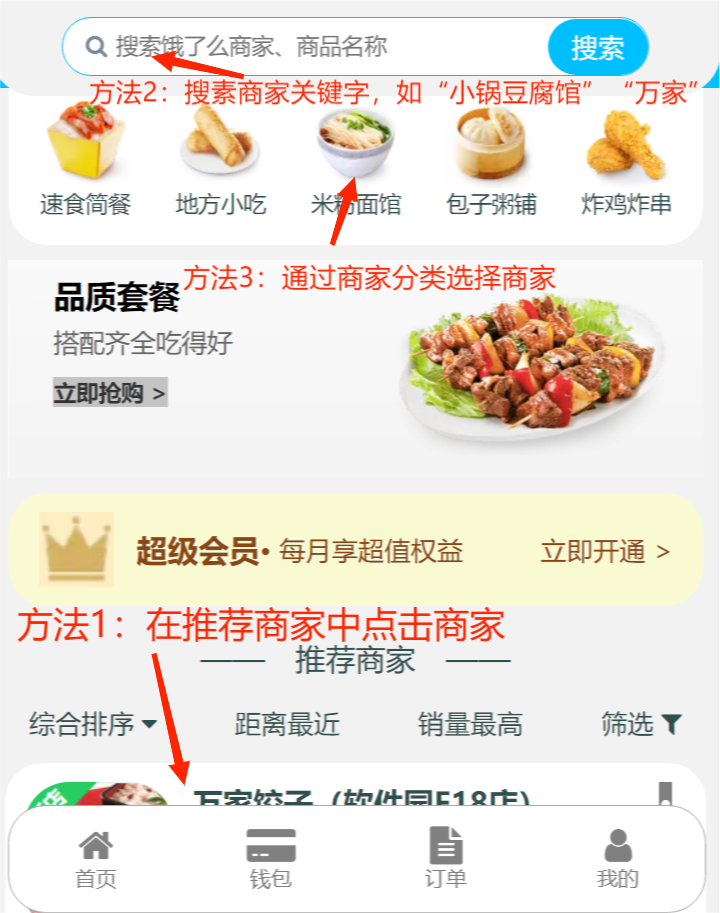
\includegraphics[width=\textwidth,height=0.3\textheight]{order1}
        \caption{选择商家的三种方法}\label{fig:order1}
    \end{minipage}
    \begin{minipage}{0.4\textwidth}
        \centering
        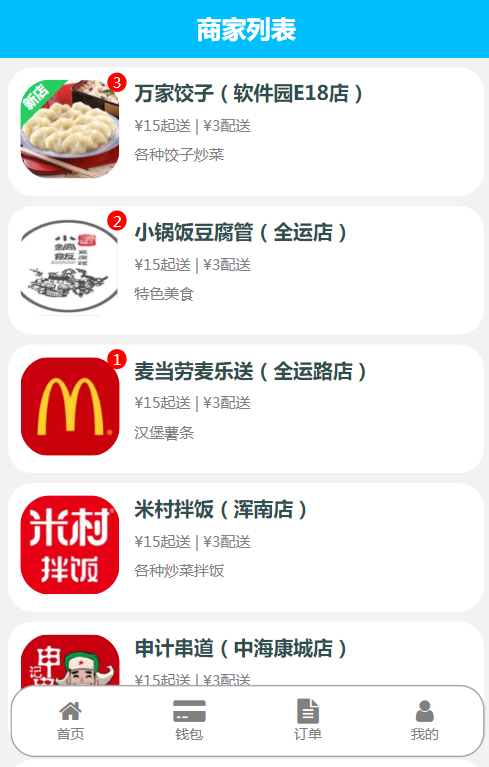
\includegraphics[width=\textwidth,height=0.3\textheight]{businessList}
        \caption{进入商家列表}\label{fig:businessList}
    \end{minipage}
    \vspace{\baselineskip}
\end{figure}

其次,进入商家后,用户可以在商家信息中进行点餐,点击“+”增加数量,点击“-”减少数量。最后点击“去结算”,此时,若用户未登录,则页面跳转至登录页面,用户可进行登录或注册操作。登陆成功后,页面重新返回,再次点击“去结算”,跳转至确认订单页面。如图~\ref{fig:order3}所示。
\begin{figure}[htbp]
    \centering
    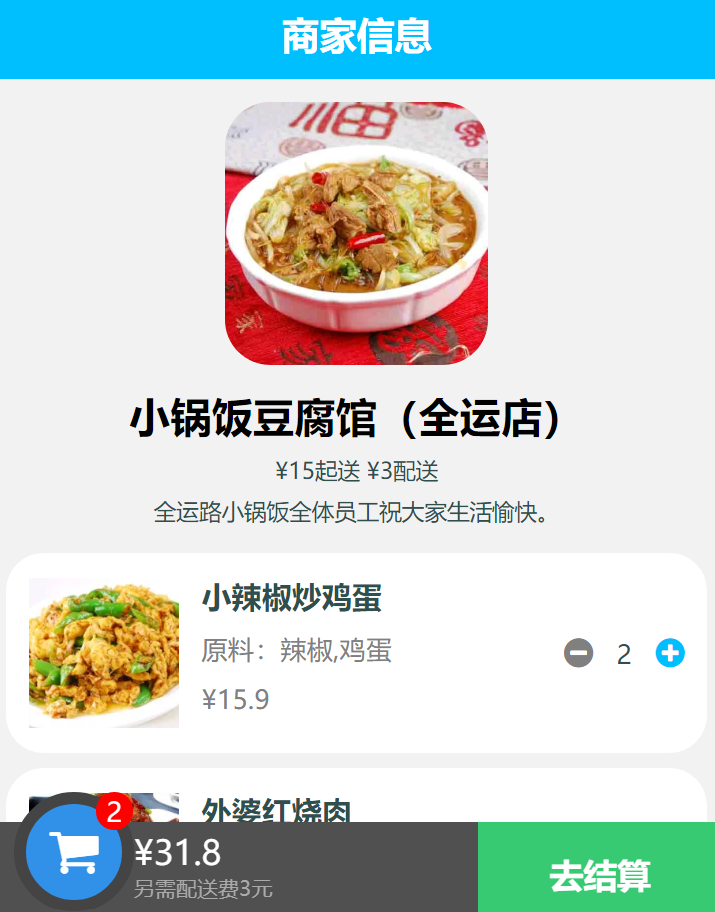
\includegraphics[width=0.4\textwidth,height=0.3\textheight]{order3}
    \caption{进入商家信息并点餐}\label{fig:order3}
\end{figure}

在确认订单页面,点击配送地址部分,可跳转至地址管理页面,对地址进行修改、删除或添加。然后点击去支付,进入支付页面。如图~\ref{fig:order5}~和~\ref{fig:userAddress}~所示.
\begin{figure}[htbp]
    \centering
    \begin{minipage}{0.4\textwidth}
        \centering
        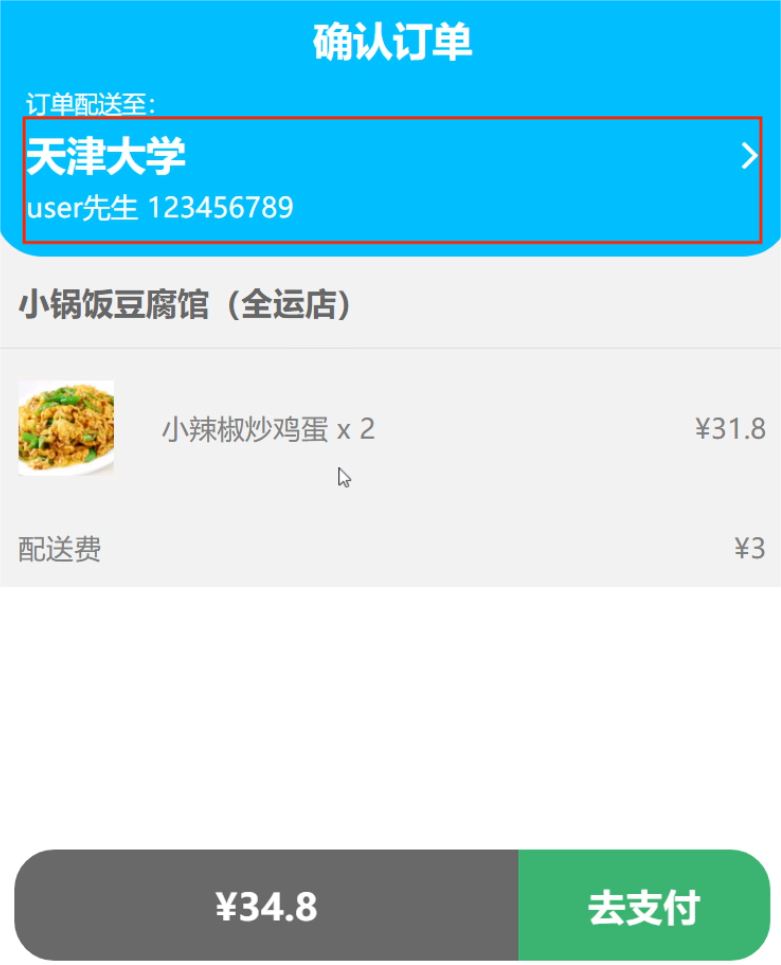
\includegraphics[width=\textwidth]{order5}
        \caption{确认订单页面}\label{fig:order5}
    \end{minipage}
    \begin{minipage}{0.4\textwidth}
        \centering
        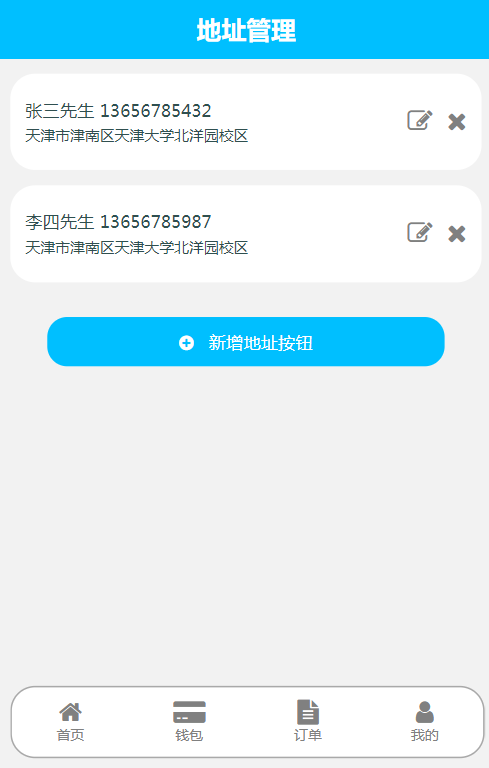
\includegraphics[width=\textwidth,height=0.3\textheight]{userAddress}
        \caption{地址管理页面}\label{fig:userAddress}
    \end{minipage}
    \vspace{\baselineskip}
\end{figure}

最后,在支付页面点击下拉按钮查看订单详情,并选择支付方式,点击“确认支付”,跳转至支付成功页面,点击“回到首页”返回首页。如图~\ref{fig:orderhidden}~和~\ref{fig:paymentDone1}~所示.

\begin{figure}[htbp]
    \centering
    \begin{minipage}{0.4\textwidth}
        \centering
        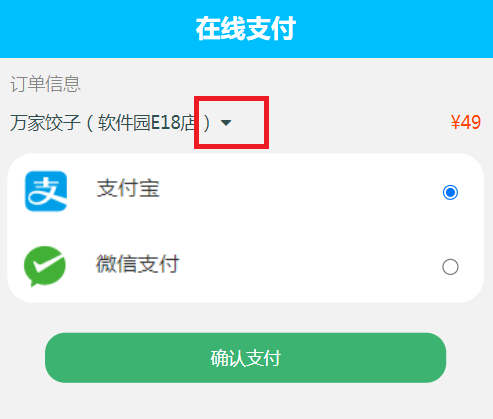
\includegraphics[width=\textwidth]{orderhidden}
        \caption{支付页面}\label{fig:orderhidden}
    \end{minipage}
    \begin{minipage}{0.4\textwidth}
        \centering
        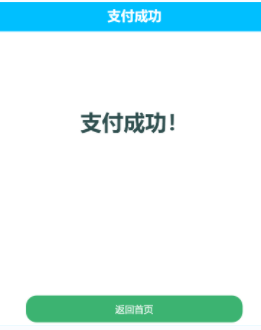
\includegraphics[width=\textwidth,height=0.25\textheight]{paymentDone1}
        \caption{支付成功页面}\label{fig:paymentDone1}
    \end{minipage}
\end{figure}
此外,针对几个重要的页面,我们对其进行了进一步的测试:
\begin{enumerate}
    \item{注册}:
    \begin{itemize}
        \item{输入数据}:手机号码:12345678911;密码:123;确认密码:111;用户名称:user;性别:女;
        \item {预期结果}:两次输入的密码不一致!
        \item {实际结果}:如图~\ref{fig:conflictingPass}~所示.
              \begin{figure}[htbp]
                  \centering
                  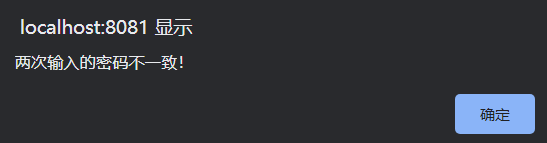
\includegraphics[width=0.6\textwidth]{conflictingPass}
                  \caption{注册密码不一致图}\label{fig:conflictingPass}
              \end{figure}
              ~\\
              \item{输入数据}:手机号码:12345678911;密码:123;确认密码:123;用户名称:user;性别:女;
        \item {预期结果}:注册成功并跳转至登录页面
        \item {实际结果}:注册成功并跳转至登录页面.如图~\ref{fig:login1}~所示.
              \begin{figure}[htbp]
                  \centering
                  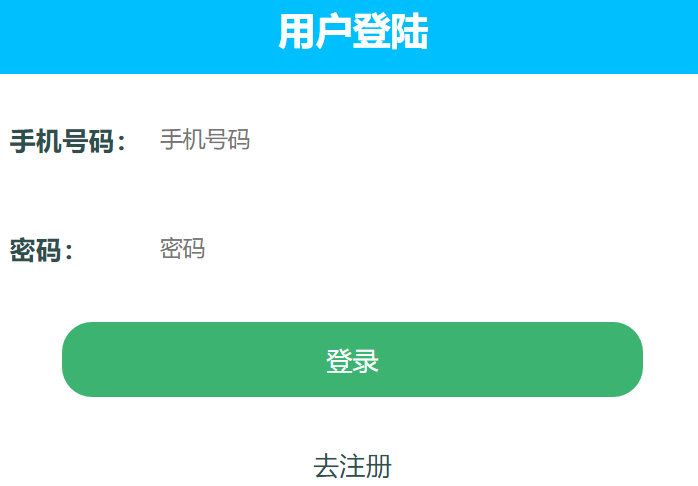
\includegraphics[width=0.4\textwidth,height=0.13\textheight]{login1}
                  \caption{注册成功返回登录的图}\label{fig:login1}
              \end{figure}
              ~\\
              \item{预置条件}:手机号12345678911已注册
              \item{输入数据}:手机号码:12345678911;密码:123;确认密码:123;用户名称:user;性别:女;
        \item {预期结果}:此手机号码已存在!
        \item {实际结果}:如图~\ref{fig:existingTel}~所示.
              \begin{figure}[htbp]
                  \centering
                  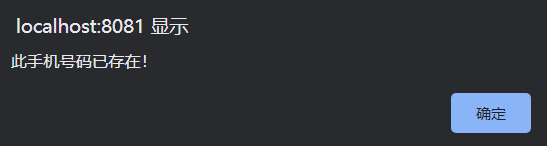
\includegraphics[width=0.5\textwidth,height=0.08\textheight]{existingTel}
                  \caption{重复注册图}\label{fig:existingTel}
              \end{figure}
    \end{itemize}
    \item {登录}:
          \begin{itemize}
              \item{预置条件}:手机号12345678911已注册
              \item{输入数据}:手机号码:12345678911;密码:123;
              \item{预期结果}:若上一个页面为注册页面,则返回首页,否则返回登录前的页面
              \item{实际结果}:当上一个页面为注册页面时,登录后仍返回注册页面
              \item{解决办法}:前端页面跳转至login前,记录来时的路由,并判断是否为register,若是,则登录成功后跳转至首页,否则跳转至来时的路由。如图~\ref{fig:beforeRouter}~和~\ref{fig:isRegister}~所示.
              \begin{figure}[htbp]
                  \centering
                  \begin{minipage}{0.4\textwidth}
                      \centering
                      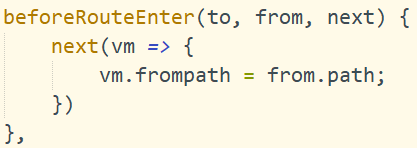
\includegraphics[width=\textwidth]{beforeRouter}
                      \caption{记录来时的路由}\label{fig:beforeRouter}
                  \end{minipage}
                  \begin{minipage}{0.4\textwidth}
                      \centering
                      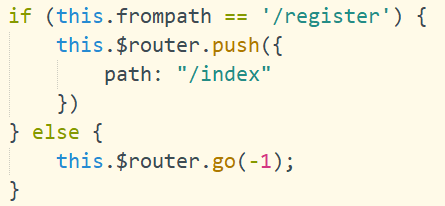
\includegraphics[width=\textwidth,height=0.095\textheight]{isRegister}
                      \caption{判断来时的路由}\label{fig:isRegister}
                  \end{minipage}                 
              \end{figure}
          \end{itemize}
    \item {“订单”页面}:
          \begin{itemize}
              \item{操作说明}:点击下拉按钮查看订单详情,点击“去支付”支付订单
              \item {预期结果}:可以看到点餐详情,“去支付”后跳转至支付页面
              \item {实际结果}:如图~\ref{fig:detail}~和~\ref{fig:orderhidden}~所示.
                    \begin{figure}[htbp]
                        \centering
                        \begin{minipage}{0.35\textwidth}
                            \centering
                            \includegraphics[width=\textwidth,height=0.1\textheight]{detail}
                            \caption{订单详情}\label{fig:detail}
                        \end{minipage}
                        \begin{minipage}{0.35\textwidth}
                            \centering
                            \includegraphics[width=\textwidth,height=0.1\textheight]{orderhidden}
                            \caption{去支付}\label{fig:orderhidden}
                        \end{minipage}
                        \vspace{\baselineskip}
                    \end{figure}
          \end{itemize}

    \item {“我的”页面}:
          \begin{itemize}
              \item{操作说明}:点击用户名旁的编辑按钮,更改用户名为“张三”
              \item {预期结果}:“我的”页面用户名更改为“张三”
              \item {实际结果}:数据库用户名更改成功,但“我的”页面用户名仍为原用户名
              \item {解决办法}:向sessionStorage中存储新的user对象。如图~\ref{fig:setNewName}~和~\ref{fig:updateName}~所示.
          \end{itemize}
          \begin{figure}[htbp]
            \centering
            \begin{minipage}{0.4\textwidth}
                \centering
                \includegraphics[width=\textwidth]{setNewName}
                \caption{SessionStorage修改}\label{fig:setNewName}
            \end{minipage}
            \begin{minipage}{0.4\textwidth}
                \centering
                \includegraphics[width=\textwidth]{updateName}
                \caption{更改用户名成功图}\label{fig:updateName}
            \end{minipage}
        \end{figure}
          \begin{itemize}
              \item{操作说明}:点击“修改密码”,第一次在“旧密码”中输入错误密码;第二次在“旧密码”中输入正确密码。
              \item {预期结果}:第一次修改密码失败;第二次修改密码成功。
              \item {实际结果}:第一次修改密码失败;第二次修改密码成功。如图~\ref{fig:errorPass}~和~\ref{fig:correctPass}~所示.
          \end{itemize}
          \begin{figure}[htbp]
              \centering
              \begin{minipage}{0.4\textwidth}
                  \centering
                  \includegraphics[width=\textwidth]{errorPass}
                  \caption{更改密码失败图}\label{fig:errorPass}
              \end{minipage}
              \begin{minipage}{0.4\textwidth}
                  \centering
                  \includegraphics[width=\textwidth]{correctPass}
                  \caption{更改密码成功图}\label{fig:correctPass}
              \end{minipage}
          \end{figure}
          \begin{itemize}
              \item{操作说明}:点击“我的地址”
              \item {预期结果}:进入“地址管理”页面,可进行地址的增删改
              \item {实际结果}:完成“地址管理”页面中地址的增删改功能。如图~\ref{fig:address}~所示.
          \end{itemize}
          \begin{figure}[htbp]
              \centering
              \includegraphics[width=0.4\textwidth]{address}
              \caption{地址管理}\label{fig:address}
          \end{figure}
          \begin{itemize}
              \item{操作说明}:点击“退出登录”
              \item {预期结果}:返回登录页面,用户再次访问时需登录认证
              \item {实际结果}:返回登录页面,但用户再次访问时仍保持登录状态
              \item {解决办法}:在退出登录后,前端需要从sessionStorage中移除user对象。如图~\ref{fig:withdrew}~所示.
          \end{itemize}
          \begin{figure}[htbp]
              \centering
              \includegraphics[width=0.4\textwidth]{withdrew}
              \caption{退出登录}\label{fig:withdrew}
          \end{figure}

\end{enumerate}

\section{部署}
\begin{itemize}
    \item{开发工具}:hbuilder、STS(spring-tool-suite)、Tomcat8.5、mysql-5.5.62-winx64
    \item {前端部署}:
          \begin{itemize}
              \item 安装 Node.js、Vue-Cli
              \item 打开hbuilder,点击文件-导入-从本地目录导入,将前端工程导入到 hbuilder 中
              \item 在cmd中,使用cd命令切换到项目路径下,使用命令npm install安装依赖, 安装成功后,在项目文件夹下出现 node\_modules 文件夹,里面是项目依赖
              \item 输入命令 npm run serve 启动项目,在浏览器中输入网址 $http://localhost:8081$,进入首页
          \end{itemize}
    \item {后端部署}:
          \begin{itemize}
              \item 安装 jdk、STS、Tomcat、MySql
              \item 在 mysql 数据库中创建数据库 elm,使用数据库脚本 elm.sql 创建数据库和初始数据
              \item 在 STS 中导入 elm 项目,并部署到 Tomcat 中
              \item 打开 com/neusoft/elm/util/dbcp.properties 修改数据库密码
              \item 在Servers上启动Tomcat
          \end{itemize}
\end{itemize}

 %第三项目
	%\chapter{SpringBoot~项目}
\section{整体概述}
本部分是使用SpringBoot重构整个项目的后端部分。目的是提供一套完整正确的用户点餐后端程序,和一套完备的可拓展可维护的后端结构。

\section{项目技术架构}
JDK17 MySQL SpringBoot Maven3.6.3

\section{设计}

\subsection{模块设计}
四个阶段的项目加上组内实现的创新和优化,代码共计四万余行,为了应对庞大的工程量以及确保项目的可维护性与可拓展性,我们采用了模块化设计的方法。各个模块被设计为相对独立的单元,为了满足高内聚低耦合的特性。在模块划分上,整个项目沿用了~SpringBoot~框架的分层架构,按照以下的方式组织。
\begin{figure}[htbp]
    \centering
    \includegraphics[width=0.8\textwidth]{elm_springboot_framework}
    \caption{项目结构模块设计}\label{fig:elm_springboot_framework}
    \vspace{\baselineskip}
\end{figure}

\subsubsection{表现层~(Presentation Layer)~}
表示层通常负责应用程序的用户界面部分,用于与用户进行交互和处理用户用户请求。它通常包括控制器~(Controller)~或路由~(Router)~层,这些组件接收来自前端或其他客户端的请求,并将它们路由到适当的处理程序。在本项目中,表示层由前端项目负责实现,后端只负责提供接口。在前端项目中,我们使用~Vue3~框架,主要的内容和部分都在上文已有介绍,在这里不做赘述。

\subsubsection{业务层~(Service Layer)~}
业务层是整个模块的核心部分,负责处理业务逻辑和业务规则。在本项目中,业务层由~SpringBoot~项目负责实现。在业务层中,我们使用了~Spring~框架提供了依赖注入和事务管理等丰富的特性,可以有助于简化业务逻辑的编写和管理。

\subsubsection{持久层~(Persistence Layer)~}
持久层负责与后端数据存储进行交互,在本项目中,使用~Spring~框架提供的对于~MySQL~数据库的数据访问技术支持,如JDBC等。在这一层,本项目定义了数据访问对象~(Dao)~来执行数据库操作。

\subsubsection{模型层~(Module Layer)~}
模型层是应用程序的数据表示层。它包括实体~(Entry)~或~(POJO)~类,这些类通常用于表示应用程序中的数据结构。模型层的对象通常与数据库表之间崔在因施工和关系,这些由数据访问层负责管理。

\subsection{数据库设计}

\subsubsection{后台管理数据库设计}
由于阶段一要实现饿了么管理员对于每一\begin{table}[htbp]
    \caption{商家列表}\label{tab:table_6_1}
    \vspace{0.5em}\wuhao
    \begin{tabularx}{\hsize}{@{\extracolsep{\fill}}c c c}
    \toprule[1.5pt]
    字段名          & 数据类型  & 说明 \\ 
    \midrule[1pt]
    businessId      & int      & 商家编号 \\
    password        & varchar  & 密码 \\
    businessName    & varchar  & 商家名称 \\
    businessAddress & varchar  & 商家地址 \\
    businessExplain & varchar  & 商家介绍 \\
    starPrice       & decimal  & 起送费 \\
    deliveryPrice   & decimal  & 配送费 \\
    \bottomrule[1.5pt]
    \end{tabularx}
\vspace{\baselineskip}
\end{table}个商家得管理,每个商家又要对自身的基本信息(例如起送费、配送费)进行管理。因此我们要有一张商家表以及管理员表。商家表的设计如表\ref{tab:table_6_1} 所示,管理员表的设计如表\ref{tab:table_6_2}所示。这里特别需要提出的是,由于起送费和配送费小数点后边不会超过两位,我们这里特地把~starPrice~和~deliveryPrice~字段的数据类型设置为~decimal~。



\begin{table}[htbp]
    \caption{管理员表}\label{tab:table_6_2}
    \vspace{0.5em}\wuhao
    \begin{tabularx}{\hsize}{@{\extracolsep{\fill}}c c c}
    \toprule[1.5pt]
    字段名          &  数据类型  &   说明 \\ 
    \midrule[1pt]
    adminId      & int     & 管理员编号 \\
    adminName   & varchar  & 管理员名称 \\
    password    & varchar  & 密码   \\

    \bottomrule[1.5pt]
    \end{tabularx}
\vspace{\baselineskip}
\end{table}

又由于每个商家要对自身出售的商品进行管理,因此我们需要一个食品表。食品表的设计如表\ref{tab:table_6_3} 所示。同样由于食品价格小数点后边不会超过两位,我们这里特地把~foodPrice~字段的数据设置为~decimal~。同时~businessId~字段为~buisiness~表的~businessId~字段的外键。

\begin{table}[htbp]
    \caption{食品表}\label{tab:table_6_3}
    \vspace{0.5em}\wuhao
    \begin{tabularx}{\hsize}{@{\extracolsep{\fill}}c c c}
    \toprule[1.5pt]
    字段名          &  数据类型  &   说明 \\ 
    \midrule[1pt]
    foodId      & int     & 食品编号 \\
    foodName   & varchar  & 食品名称 \\
    foodExplain    & varchar  & 食品介绍   \\
    foodPrice      & decimal     & 食品价格 \\
    businessId      & int     & 所属商家编号 \\
    \bottomrule[1.5pt]
    \end{tabularx}
\vspace{\baselineskip}
\end{table}

\subsubsection{点餐业务数据库设计}

点餐业务中需要记录每一个用户的信息,以便实现登录历史订单查询等功能,需要一个用户表来记录每一个用户的信息。用户表的设计如表\ref{tab:table_6_4} 所示。

\begin{table}[htbp]
    \caption{用户表}\label{tab:table_6_4}
    \vspace{0.5em}\wuhao
    \begin{tabularx}{\hsize}{@{\extracolsep{\fill}}c c c}
    \toprule[1.5pt]
    字段名          &  数据类型  &   说明 \\ 
    \midrule[1pt]
    userId      & varchar     & 食品编号 \\
    password   & varchar  & 食品名称 \\
    userName    & varchar  & 食品介绍   \\
    userSex      & int     & 食品价格 \\
    userImg      & mediumtext     & 所属商家编号 \\
    delTag      & int     & 所属商家编号 \\
    \bottomrule[1.5pt]
    \end{tabularx}
\vspace{\baselineskip}
\end{table}

点餐业务中需要向用户展示全部的商家信息,所以我们需要有一张商家表。每个商家又需要向顾客展示所售卖的全部食物,于是需要有一张食品表。其中食品表中的~businessId~字段是食品表中的~businessId~字段的外键。商家表的设计如表\ref{tab:table_6_5},食品表的设计如表\ref{tab:table_6_6}所示。

\begin{table}[htbp]
    \caption{商家表(点餐业务)}\label{tab:table_6_5}
    \vspace{0.5em}\wuhao
    \begin{tabularx}{\hsize}{@{\extracolsep{\fill}}c c c}
    \toprule[1.5pt]
    字段名          &  数据类型  &   说明 \\ 
    \midrule[1pt]
    businessId   & int  & 商家编号 \\
    businessName    & varchar  & 商家名称   \\
    businessAddress  & varchar & 商家地址 \\
    businessExplain     & varchar     & 商家介绍 \\
    businessImg      & mediumtext     & 商家图片 \\
    orderTypeId      & int     & 共用10种点餐分类 \\
    starPrice      & decimal     & 起送费 \\
    deliveryPrice      & decimal     & 配送费 \\
    remarks     & varchar     & 备注 \\
    \bottomrule[1.5pt]
    \end{tabularx}
\vspace{\baselineskip}
\end{table}

\begin{table}[htbp]
    \caption{食品表(点餐业务)}\label{tab:table_6_6}
    \vspace{0.5em}\wuhao
    \begin{tabularx}{\hsize}{@{\extracolsep{\fill}}c c c}
    \toprule[1.5pt]
    字段名          &  数据类型  &   说明 \\ 
    \midrule[1pt]
    foodId      & int     & 食品编号 \\
    foodName   & varchar  & 食品名称 \\
    foodExplain    & varchar  & 食品介绍   \\
    foodImg      & mediumtext     & 食品图片 \\
    foodPrice      & decimal     & 食品价格 \\
    businessId      & int     & 所属商家编号 \\
    businessId      & varchar     & 备注 \\
    \bottomrule[1.5pt]
    \end{tabularx}
\vspace{\baselineskip}
\end{table}

又由于要实现用户能够选购商品的功能,需要有一个购物车表来记录用户在特定商家所选购的商品。购物车表中的~foodId~字段为食品表中~foodId~字段的外键,~businessId~字段为商家表中~businessId~的外键,~userId~字段为用户表中~userId~字段的外键。购物车表的设计如表\ref{tab:table_6_7}所示。

\begin{table}[htbp]
    \caption{购物车表}\label{tab:table_6_7}
    \vspace{0.5em}\wuhao
    \begin{tabularx}{\hsize}{@{\extracolsep{\fill}}c c c}
    \toprule[1.5pt]
    字段名          &  数据类型  &   说明 \\ 
    \midrule[1pt]
    cardId      & int     & 无意义编号 \\
    foodId   & int  & 食品名称 \\
    businessId    & int  & 所属商家编号   \\
    userId      & varchar     & 所属用户编号 \\
    quantity      & int     & 同一类型食品的购买数量 \\
    \bottomrule[1.5pt]
    \end{tabularx}
\vspace{\baselineskip}
\end{table}

每一个用户都有不同的送货地址,所以我们需要一个送货地址表来记录每
一个用户所对应的配送地址,送货地址表中的~userId~字段为用户表中的~userId~字
段的外键。送货地址表的设计如表\ref{tab:table_6_8}所示。

\begin{table}[htbp]
    \caption{送货地址表}\label{tab:table_6_8}
    \vspace{0.5em}\wuhao
    \begin{tabularx}{\hsize}{@{\extracolsep{\fill}}c c c}
    \toprule[1.5pt]
    字段名          &  数据类型  &   说明 \\ 
    \midrule[1pt]
    daId      & int     & 送货地址编号 \\
    contactName   & varchar  & 联系人姓名 \\
    contactSex    & int  & 联系人性别   \\
    contactTel   & varchar     & 联系人电话 \\
    address      & varchar     & 送货地址 \\
    userId      & varchar     & 所属用户编号 \\
    \bottomrule[1.5pt]
    \end{tabularx}
\vspace{\baselineskip}
\end{table}

用户选购完商品之后,需要能够进行对购物车中所选购的商品进行下单,这就需要一个订单表和一个订单明细表。订单表中的~userId~字段为用户表中的~userId~字段的外键,~businessId~字段为商家表中~businessId~字段的外键,~daId~字段为送货地址表中~daId~字段的外键。订单明细表中的~orderId~字段为订单表中的~orderId~字段的外键,~foodId~字段为食品表中~foodId~字段的外键。订单表的具体实现如表\ref{tab:table_6_9}所示,~订单明细表的具体实现如表\ref{tab:table_6_10}所示。

\begin{table}[htbp]
    \caption{订单表}\label{tab:table_6_9}
    \vspace{0.5em}\wuhao
    \begin{tabularx}{\hsize}{@{\extracolsep{\fill}}c c c}
    \toprule[1.5pt]
    字段名          &  数据类型  &   说明 \\ 
    \midrule[1pt]
    orderId      & int     & 订单编号 \\
    userId   & varchar  & 所属用户编号 \\
    businessId    & int  & 所属商家编号   \\
    orderDate   & varchar     & 订购日期 \\
    orderTotal      & decimal     & 订单总价 \\
    daId      & int     & 所属送货地址编号 \\
    orderState      & int     & 订单状态(0未支付,1已支付) \\
    \bottomrule[1.5pt]
    \end{tabularx}
\vspace{\baselineskip}
\end{table}

\begin{table}[htbp]
    \caption{订单明细表}\label{tab:table_6_10}
    \vspace{0.5em}\wuhao
    \begin{tabularx}{\hsize}{@{\extracolsep{\fill}}c c c}
    \toprule[1.5pt]
    字段名          &  数据类型  &   说明 \\ 
    \midrule[1pt]
    odId      & int     & 订单明细编号 \\
    orderId   & int  & 所属订单编号 \\
    foodId    & int  & 所属食品编号   \\
    quantity   & int     & 数量 \\
    \bottomrule[1.5pt]
    \end{tabularx}
\vspace{\baselineskip}
\end{table}

\subsection{接口设计}

\subsubsection{外部接口}
用户或其他软件可以通过~Interne~访问服务器~IP~实现对本软件的访问。同时提供图形化UI界面供用户使用。并且提供其他软件能够访问本项目的接口。网络传输协议采用HTTP协议,具体使用方法为:~http://IP地址/数据库名/内部接口~

\subsubsection{内部接口}
内部接口主要是为了实现软件的功能,提供给前端调用。内部接口的具体实现如下所示。

接口的部分已经在第三部分Serverlet部分阐述过,这里不做赘述。


\section{点赞业务流后端的SpringBoot实现}
点餐业务流后端采用~SpringBoot+Mybatis~实现,利用~Mybatis~连接并操作数据库,使得对于数据库的操作代码编写简单。~SpringBoot~框架采用三层架构,即控制层、业务层和持久层。控制层向上层即前端提供接口,使得前端可以调用后端接口;业务层实现具体业务代码,如数据库的事务型操作在这里体现;持久层即编写~SQL~语句操作数据库,实现对数据库的修改和访问。三层架构中,除持久层外,其余层代码较为简单,大致模板如下,除部分业务代码外不再给出具体实现:

\begin{lstlisting}[basicstyle=\footnotesize]
//控制层代码模板
@RestController
@RequestMapping("/XXXXController")
public class XXXXController {
    
    @Autowired
    private XXXXService xxxxService;

    @RequestMapping("接口名/")
    public 返回值类型接口名参数类型( 参数名)throws Exception{
        return xxxxService接口名参数名.();
    }
    
    ...
}
\end{lstlisting}

\begin{lstlisting}[basicstyle=\footnotesize]
//业务层接口代码模板
public interface XXXXService {
    public 返回值类型接口名参数类型( 参数名);
    ...
}
\end{lstlisting}

\begin{lstlisting}[basicstyle=\footnotesize]
//业务层实现代码模板
@Service
public class XXXXServiceImpl implements XXXXService{
    @Autowired
    private XXXXMapper xxxxMapper;
    @Override
    public 返回值类型接口名参数类型( 参数名) {
        return xxxxMapper接口名参数名.();
    }
    ...
}
\end{lstlisting}

其中,“XXXX”为对应的类,详见图\ref{fig:table_forSB}.
点餐业务流共涉及对客户表、地址表、商家表、食品表、购物车表、订单
表和订单明细表的修改与访问,具体如下。

\begin{figure}[htbp]
    \centering
    \includegraphics[width=0.8\textwidth]{table_forSB}
    \caption{点餐业务流SpringBoot实现类}\label{fig:table_forSB}
    \vspace{\baselineskip}
\end{figure}

\section{用户信息模块功能实现}
本模块,涉及对用户表和地址表的修改与访问。~SQL~语句较为简单、因此采用注解的方式直接写在~Java~代码中。

\begin{lstlisting}[basicstyle=\footnotesize]
//对表的修改与查询User
@Mapper
public interface UserMapper {
    @Select("select * from user where userId=#{userId} and
        password=#{password}")
    public User getUserByIdByPass(User user);
    @Select("select count(*) from user where userId=#{userId}")
    public int getUserById(String userId);
    @Insert("insert into user
        values(#{userId},#{password},#{userName},#{userSex},null,1)")
    public int saveUser(User user);
}
\end{lstlisting}


\begin{lstlisting}[basicstyle=\footnotesize]
//对地址表的修改与查询
@Mapper
public interface DeliveryAddressMapper {
    @Select("select * from deliveryAddress where userId=#{userId} 
        order by daId")
    public List<DeliveryAddress> listDeliveryAddressByUserId(String
        userId);
    @Select("select * from deliveryAddress where daId=#{daId}")
    public DeliveryAddress getDeliveryAddressById(Integer daId);
    @Insert("insert into deliveryAddressvalues(null,#{contactName},
        #{contactSex},#{contactTel},#{address},#{userId})")
    public int saveDeliveryAddress(DeliveryAddress deliveryAddress);
    @Update("update deliveryAddress set contactName=#{contactName}
        ,contactSex=#{contactSex},contactTel=#{contactTel},
        address=#{address}where daId=#{daId}")
    public int updateDeliveryAddress(DeliveryAddress 
        deliveryAddress);
    @Delete("delete from deliveryAddress where daId=#{daId}")
    public int removeDeliveryAddress(Integer daId);
}
\end{lstlisting}

\section{商家信息模块}
本模块涉及对商家表和食品表的修改与访问。简单的 SQL 语句不再给出实现,部分较为复杂的 SQL 语句写在 XML 文件中,如模糊查询、参数不定等。

\begin{lstlisting}[basicstyle=\footnotesize]
SELECT * FROM (
    SELECT COUNT(o.orderId)
        num,b.businessId,b.businessAddress,b.businessExplain,
        b.businessImg,b.businessName,b.deliveryPrice,
        b.orderTypeId,b.remarks,b.starPrice,o.orderId
    FROM business b LEFT OUTER JOIN (
        SELECT orders.businessId,orders.orderId FROM orders WHERE
        orders.userId=#{userId}
    ) o
    ON o.businessId = b.businessId GROUP BY b.businessId) a
ORDER BY a.num DESC
\end{lstlisting}

\section{点单业务模块}
本模块涉及对购物车表、订单表和订单明细表的修改与访问。在创建订单时涉及到事务,即要么不执行,要么全部执行。在~SpringBoot~框架中使用注解
~“@Transactional”~说明某方法是一个事务。

\begin{lstlisting}[basicstyle=\footnotesize]
@Service
public class OrdersServiceImpl implements OrdersService{
    private CartMapper cartMapper;
    @Autowired
    private OrdersMapper ordersMapper;
    @Autowired
    private OrderDetailetMapper orderDetailetMapper;
    @Override
    @Transactional
    public int createOrders(Orders orders) {
        //查询当前用户购物车中当前商家的所有食品1.
        Cart cart = new Cart();
        cart.setUserId(orders.getUserId());
        cart.setBusinessId(orders.getBusinessId());
        List<Cart> cartList = cartMapper.listCart(cart);
        //创建订单(返回生成的订单编号)2.
        orders.setOrderDate(CommonUtil.getCurremntDate());
        ordersMapper.saveOrders(orders);
        int orderId = orders.getOrderId();
        //批量添加订单明细3.
        List<OrderDetailet> list = new ArrayList<>();
        for(Cart c : cartList) {
            OrderDetailet od = new OrderDetailet();
            od.setOrderId(orderId);
            od.setFoodId(c.getFoodId());
            od.setQuantity(c.getQuantity());
            list.add(od);
        }
        orderDetailetMapper.saveOrderDetailetBatch(list);
        //从购物车表中删除相关食品信息4.
        cartMapper.removeCart(cart);
        return orderId;
    }
}
\end{lstlisting}

此外,在访问订单是,涉及到多表查询,即订单表连接订单明细表,订单表用于连接到商家表,~XML~的实现如下:

\begin{lstlisting}[basicstyle=\footnotesize]
<resultMap type="com.kbz320.elmboot.po.Orders" id="ordersResultMap">
    <id column="orderId" property="orderId"/>
    <result column="userId" property="userId"/>
    <result column="businessId" property="businessId"/>
    ...
    <association property="business"
        javaType="com.kbz320.elmboot.po.Business"
        select="com.kbz320.elmboot.mapper.BusinessMapper.getBusinessById"column="businessId"/>
    <collection property="list"
        ofType="com.kbz320.elmboot.po.OrderDetailet"
        select="com.kbz320.elmboot.mapper.OrderDetailetMapper.listOrderDetailetByOrderId"column="orderId"/>
</resultMap>

<select id="getOrdersById" parameterType="java.lang.Integer"
    resultMap="ordersResultMap">
    select * from orders where orderId=#{orderId}
</select>

<select id="listOrdersByUserId" parameterType="java.lang.String"
    resultMap="ordersResultMap">
    select * from orders where userId=#{userId}
</select>
\end{lstlisting}

其中,"association"表示一对一连接,而"collection"表示一对多连接。

\section{测试}
此次项目,我们依旧对正常点餐流程、“注册” “登录” “订单” “我的”等页面进行了测试,具体测试过程与servlet项目中的“测试”部分一致。

此外,由于新增了积分系统,我们对其进行了单独的功能测试,具体结果如下。~\\
\subsection{积分支付选择}
“在线支付”页面中,系统会根据用户的订单金额和剩余积分,按照最优原则,尽可能最大化用户抵扣金额,减少支付金额。支付时,用户可以自行选择是否使用积分,再点击“确认支付”。如图~\ref{fig:creditPay}~所示。
支付时,若余额不足,会显示“您没钱了,请去充值!”,然后跳转至“钱包”页面,充值后即可再次支付。如图~\ref{fig:noMoney}~所示。~\\
\begin{figure}[htbp]
    \centering
    \begin{minipage}{0.4\textwidth}
        \centering
        \includegraphics[width=\textwidth]{creditPay}
        \caption{积分支付页面}\label{fig:creditPay}
    \end{minipage}
    \begin{minipage}{0.4\textwidth}
        \centering
        \includegraphics[width=\textwidth,height=0.3\textheight]{noMoney}
        \caption{余额不足}\label{fig:noMoney}
    \end{minipage}
    \vspace{\baselineskip}
\end{figure}
\begin{itemize}
    \item {使用积分支付}:支付成功后,返回“钱包”页面,发现积分被抵扣了,余额减少的部分为订单金额-抵扣金额,点击“积分明细”,也有相应的积分消费记录。如图~\ref{fig:creditPayment}~所示~\\
    \begin{figure}[htbp]
        \centering
        \includegraphics[width=0.8\textwidth]{creditPayment}
        \caption{积分支付详情}\label{fig:creditPayment}
        \vspace{\baselineskip}
    \end{figure}

    \item {不使用积分支付}:支付成功后,返回“钱包”页面,发现积分没有变动,余额减少的部分为订单金额数。如图~\ref{fig:notCredit}~所示~\\
    \begin{figure}[htbp]
        \centering
        \includegraphics[width=0.9\textwidth,height=0.25\textheight]{notCredit}
        \caption{不使用积分支付详情}\label{fig:notCredit}
        \vspace{\baselineskip}
    \end{figure}
\end{itemize}
\subsection{“钱包”页面}
\begin{enumerate}
\item {充值提现}:输入操作金额后,点击“充值”或“提现”,即可进行操作,若无操作金额或为负数,显示“充值(或提现)金额错误”。如图~\ref{fig:errorMoney}~所示。若充值成功,则更新钱包页面的金额、积分数量。如图~\ref{fig:recharge}~所示。
\begin{figure}[htbp]
    \centering
    \includegraphics[width=0.6\textwidth]{errorMoney}
    \caption{操作金额错误时报错}\label{fig:errorMoney}
\end{figure}
\begin{figure}[htbp]
    \centering
    \includegraphics[width=0.6\textwidth]{recharge}
    \caption{充值成功前后对比}\label{fig:recharge}
\end{figure} 
\item {积分明细}:点击“积分明细”,可以查看获取或消费积分记录,积分来源,创建或过期时间。如图~\ref{fig:creditDetail}~所示。
\begin{figure}[htbp]
    \centering
    \includegraphics[width=0.8\textwidth,height=0.25\textheight]{creditDetail}
    \caption{查看积分明细}\label{fig:creditDetail}
\end{figure} 
\item {签到领积分}:点击“今天签到可以拿10积分”,可以领取积分,且一天只能领一次。如图~\ref{fig:sign}~所示。
\begin{figure}[htbp]
    \centering
    \includegraphics[width=0.8\textwidth,height=0.25\textheight]{sign}
    \caption{签到前后对比}\label{fig:sign}
\end{figure} 
\end{enumerate}

\section{服务器部署}
\subsection{环境}
\subsubsection{服务器选择}
阿里云服务器(2核4G centos系统) 

\subsubsection{服务器环境配置}
MySQL8.0 nginx	redis jdk17

\subsection{项目部署过程}
\subsubsection{后端部署}
修改springboot配置文件,将localhost改为服务器内网IP
\begin{figure}[htbp]
	\centering
	\includegraphics[width=0.8\textwidth]{aliyunsjk}
	\caption{修改url}
	\vspace{\baselineskip}
\end{figure}

将springboot程序打包成jar包,通过脚本运行
\begin{figure}[htbp]
	\centering
	\includegraphics[width=0.8\textwidth]{jiaoben}
	\caption{sh脚本}
	\vspace{\baselineskip}
\end{figure}
通过netstat命令查看运行情况,运行结果如下:

\begin{figure}[htbp]
	\centering
	\includegraphics[width=0.8\textwidth]{jar}
	\caption{运行情况}
	\vspace{\baselineskip}
\end{figure}

\subsubsection{前端部署}
将前端项目打包成dist文件放在home目录。

修改nginx.conf配置文件如图6-14所示
\begin{figure}[htbp]
	\centering
	\includegraphics[width=0.8\textwidth]{nginx}
	\caption{nginx配置文件修改}
	\vspace{\baselineskip}
\end{figure}

\subsubsection{最终合并}
重启nginx,同时禁止80端口和8081端口的防火墙,现在前后端就可以进行交互了。

输入服务器公网IP就能进入网页进行操作,最终效果如图6-15所示。
\begin{figure}[htbp]
	\centering
	\includegraphics[width=0.8\textwidth]{result}
	\caption{最终效果}
	\vspace{\baselineskip}
\end{figure} %第四项目
	% \chapter{项目特色之处} %项目特色
	% \chapter{总结}

\section{项目中遇到的问题及解决方法}

\section{项目开发过程}
\subsection{项目共享仓库}
我们对于本实践项目使用 GITHUB 进行仓库共享,让每一名组员可以在该仓库上进行代码的修改以及同步,大幅度增加实践效率。通过以下网址,可以游览到本项目的共享仓库页面:https://github.com/stainsatin/elm
\begin{figure}[htbp]
    \centering
    \includegraphics[width=0.8\textwidth]{githubmain}
    \caption{GITHUB 共享仓库页面}\label{fig:githubmain}
    \vspace{\baselineskip}
\end{figure}

本次实践项目的共享仓库于 8 月 23 日创建,仓库里的成员包括我们每一名组员。如上图~\ref{fig:githubmain}~所示,仓库里的内容包括本次实践项目的前端、后端与实践报告的目录,且我们每一名组员都在此共享仓库上进行了多次代码的复制和提交。经过三个星期的项目开发,以下是我们的共享仓库数据视图,如图~\ref{fig:commit}~至图所示:

\begin{figure}[htbp]
    \centering
    \includegraphics[width=0.7\textwidth]{commit}
    \caption{GITHUB 共享仓库提交视图}\label{fig:commit}
    \vspace{\baselineskip}
\end{figure}
\begin{figure}[htbp]
    \centering
    \includegraphics[width=0.8\textwidth]{clone}
    \caption{GITHUB 共享仓库复制视图}\label{fig:clone}
    \vspace{\baselineskip}
\end{figure}
\begin{figure}[htbp]
    \centering
    \includegraphics[width=0.8\textwidth]{week1commit}
    \caption{GITHUB 共享仓库第一周提交次数视图}\label{fig:week1commit}
    \vspace{\baselineskip}
\end{figure}
\begin{figure}[htbp]
    \centering
    \includegraphics[width=0.8\textwidth]{week2commit}
    \caption{GITHUB 共享仓库第二周提交次数视图}\label{fig:week2commit}
    \vspace{\baselineskip}
\end{figure}
\begin{figure}[htbp]
    \centering
    \includegraphics[width=0.8\textwidth]{week3commit}
    \caption{GITHUB 共享仓库第三周提交次数视图}\label{fig:week3commit}
    \vspace{\baselineskip}
\end{figure}
\begin{figure}[htbp]
    \centering
    \includegraphics[width=0.7\textwidth]{codefrequency}
    \caption{GITHUB 共享仓库代码频率视图}\label{fig:codefrequency}
    \vspace{\baselineskip}
\end{figure} %总结
	% \chapter{附件}
\section{新技术学习视频截图}

\begin{figure}[htbp]
    \centering
    \includegraphics[width=0.7\textwidth]{3021244187_AI}
    \caption{3021244187 易东廷}\label{fig:3021244187_AI}
    \vspace{\baselineskip}
\end{figure}
\begin{figure}[htbp]
    \centering
    \includegraphics[width=0.8\textwidth]{3021210045_AI}
    \caption{3021210045 张中天}\label{fig:3021210045_AI}
    \vspace{\baselineskip}
\end{figure}
\begin{figure}[htbp]
    \centering
    \includegraphics[width=0.8\textwidth]{3021244259_AI}
    \caption{3021244259 张梅梅}\label{fig:3021244259_AI}
    \vspace{\baselineskip}
\end{figure}
\begin{figure}[htbp]
    \centering
    \includegraphics[width=0.8\textwidth]{6321012105_AI}
    \caption{6321012105 杜伟乐}\label{fig:6321012105_AI}
    \vspace{\baselineskip}
\end{figure}

\begin{figure}[htbp]
    \centering
    \begin{minipage}{0.4\textwidth}
        \centering
        \includegraphics[width=\textwidth]{3021244187_form}
        \caption{3021244187 易东廷}\label{fig:3021244187_form}
    \end{minipage}
    \begin{minipage}{0.4\textwidth}
        \centering
        \includegraphics[width=\textwidth]{3021210045_form}
        \caption{3021210045 张中天}\label{fig:3021210045_form}
    \end{minipage}
\end{figure}
\begin{figure}[htbp]
    \centering
    \begin{minipage}{0.4\textwidth}
        \centering
        \includegraphics[width=\textwidth]{3021244259_form}
        \caption{3021244259 张梅梅}\label{fig:3021244259_form}
    \end{minipage}
    \begin{minipage}{0.4\textwidth}
        \centering
        \includegraphics[width=\textwidth]{6321012105_form}
        \caption{6321012105 杜伟乐}\label{fig:6321012105_form}
    \end{minipage}
\end{figure}
 %附件

	% \clearpage

\end{CJK*}                                     % 结束中文字体使用
\end{document}                                 % 结束全文
